%% Some items may need adjustment from time to time; search for ``FIXME'' in this document.
\documentclass[12pt]{article}
\usepackage{fullpage}
%\usepackage{mathptmx}
\usepackage{times}
\usepackage{ifthen}
\usepackage{microtype}
\usepackage{color}
\usepackage{xspace}
\usepackage{makeidx}
\usepackage{enumitem}
\usepackage{graphicx}
\usepackage[normalem]{ulem}
\usepackage{titlesec}
\usepackage{tikz}
\usepackage[plainpages=false,debug]{hyperref} % should be last package

% Next two lines let us use \cref{} for footnote cross references
% http://tex.stackexchange.com/questions/10102/multiple-references-to-the-same-footnote-with-hyperref-support-is-there-a-bett
\usepackage{cleveref}
\crefformat{footnote}{#2\footnotemark[#1]#3}


%\usepackage{fancyhdr}
%
%\fancyfoot{}
%\fancyhead[RO,LE]{\thepage}
%\fancyhead[LO]{}
%\fancyhead[RE]{}

\setlist{nosep} % tighten itemized lists

\definecolor{diColor}{rgb}{0,0,0.8}
\definecolor{deleteColor}{rgb}{1,0,0}
\definecolor{addColor}{rgb}{0.0,0.5,0}

\definecolor{oldColor}{rgb}{0.55,0.1,0.1}
\definecolor{newColor}{rgb}{0.29,0.44,0.14}
\definecolor{provisionalColor}{rgb}{0.28,0.24,0.55}
\definecolor{fixmeColor}{rgb}{0.8,0,0}
\definecolor{voteColor}{rgb}{0.5,0,1}

\newcommand\ie{i.e.\xspace}
\newcommand\eg{e.g.\xspace}
\newcommand\etc{etc.\xspace}
%\newcommand\qe{PhD Qualifying Examination\index{PhD Qualifying Examination}\xspace}
\newcommand\qe{QE\xspace}
%\newcommand\QE{PhD Qualifying Examination\index{PhD Qualifying Examination}\xspace}
\newcommand\QE{PhD Qualifying Examination\xspace}

\newcommand\delete[1]{\color{deleteColor}\sout{\textbf{#1}}\color{black}\xspace}

\newcommand\add[1]{\color{addColor}\textbf{#1}\color{black}\xspace%
\marginpar{\color{addColor}$\Delta$\color{black}}}

%\newcommand\edited{\marginpar{\color{red}$\Delta$\color{black}}}

\newcommand{\course}[2][EMPTY]%
    {\ifthenelse%
        {\equal{#1}{EMPTY}}%
        {OCEA #2}%
        {#1 #2}%
    }

%\newcommand{\di}[2][EMPTY]%
%    {\ifthenelse%
%        {\equal{#1}{EMPTY}}%
%        {\color{diColor}#2\color{black}\index{#2}}%
%        {\color{diColor}#2\color{black}\index{#1}}%
%    } 

\newcommand{\di}[1]{#1}

\newcommand{\provisional}[1]{\color{provisionalColor}#1\color{black}\index{$>>>>$PROVISIONAL TEXT$<<<<$}}

\newcommand{\replace}[2]{\color{oldColor}\sout{#1}\color{newColor}#2\color{black}\xspace}

\newcommand{\fixme}[1]{\color{fixmeColor}$\{$#1$\}$\color{black}\index{$>>>>$FIXME$<<<<$}}

\newcommand{\vote}[1]{\color{voteColor}\{#1\}\color{black}\marginpar[$\gg$OK?]{$\ll$OK?}}

\newcommand{\mutablenum}{\arabic{mutablecount}}
\newcommand{\mutable}[1]{%
    \textbf{$\ll$#1$\gg$}%
    \marginpar[$\gg$]{%
    $\Leftarrow$\textbf{\mutablenum}\stepcounter{mutablecount}%
    }%
    }

\newcommand{\discuss}[1]{\footnote{\color{fixmeColor}#1\color{black}}\index{$>>>>$DISCUSS$<<<<$}}

% sm = supplemental material
%\newcommand{\sm}[2]{\noindent \texttt{#1}}



%\newcommand{\npara}[1]{\noindent\textbf{\thesubsection.#1}} % for numbered paragraphs of appeals section

\setlength{\parindent}{0em}
% number paragraphs
\newcommand{\parnum}{\arabic{parcount}}
\newcounter{parcount}
%\newcommand\p{\stepcounter{parcount}\leavevmode[\parnum]\hspace{0.2em}\marginpar[\hfill\parnum]{\parnum}}
\newcommand\p{\stepcounter{parcount}\leavevmode{\raisebox{0.2ex}{\scriptsize[\parnum]}}\hspace{0.2em}}
\newcommand\cp{\setcounter{parcount}{0}}
\newcounter{mutablecount}
\setcounter{mutablecount}{1}

% cav = chapter and verse. arg1=section number (roman); arg2=section name; arg3=url
\newcommand{\cav}[3]{(FGS \S#1 \textsl{#2}\footnote{\footnotesize{\url{#3}}})}

\newcommand{\furl}[2][EMPTY]%
    {\ifthenelse%
        {\equal{#1}{EMPTY}}%
        {\footnote{\footnotesize{\url{#2}}}}%
        {#1\footnote{\footnotesize{\url{#2}}}}%
    }

% Use macros to get indexing, and ensure uniform representation
%\newcommand{\supervisor}{\color{diColor}supervisor\color{black}\index{supervisor}\xspace}
\newcommand{\supervisor}{Supervisor\xspace}
%\newcommand{\curcom}{\color{diColor}Curriculum Committee\color{black}\index{Committees!Curriculum}\xspace}
\newcommand{\curcom}{Curriculum Committee\xspace}
%\newcommand{\supcom}{\color{diColor}Supervisory Committee\color{black}\index{Committees!Supervisory}\xspace}
\newcommand{\supcom}{Supervisory Committee\xspace}
%\newcommand{\gocom}{\color{diColor}Graduate Oversight Committee\color{black}\index{Committees!Graduate Oversight}\xspace}
\newcommand{\gocom}{Graduate Oversight Committee\xspace}
%\newcommand{\GC}{\index{Graduate Coordinator}Graduate Coordinator\xspace}
%\newcommand{\GC}{\color{diColor}Graduate Coordinator\color{black}\index{Graduate Coordinator}\xspace}
\newcommand{\GC}{Graduate Coordinator\xspace}
%\newcommand{\GS}{\index{Graduate Secretary}Graduate Secretary\xspace}
%\newcommand{\GS}{\color{diColor}Graduate Secretary\color{black}\index{Graduate Secretary}\xspace}
\newcommand{\GS}{Graduate Secretary\xspace}
%\newcommand{\formAPR}{\index{forms!Annual Progress Report}\color{diColor}Annual Progress Report Form\color{black}\xspace}
\newcommand{\formAPR}{Annual Progress Report Form\xspace}
%\newcommand{\formGSP}{\index{forms!Graduate Student Program}\color{diColor}Graduate Student Program Form\color{black}\xspace}
\newcommand{\formGSP}{Graduate Student Program Form\xspace}
%\newcommand{\formGSPU}{\index{forms!Graduate Student Program}\color{diColor}Graduate Student Program Update Form\color{black}\xspace}
\newcommand{\formGSPU}{Graduate Student Program Update Form\xspace}
%\newcommand{\formSPRF}{\index{forms!Supplementary Program Report}\color{diColor}Supplementary Program Report Form\color{black}\xspace}
\newcommand{\formSPRF}{Oceanography Supplementary Program Report Form\xspace}
%\newcommand{\formST}{\index{forms!Sea Time}\color{diColor}Sea Time Form\color{black}\xspace}
\newcommand{\formST}{Sea Time Form\xspace}
%\newcommand{\FGS}{\index{Faculty of Graduate Studies (\textsc{fgs})}\color{diColor}\textsc{fgs}\color{black}\xspace}
%\newcommand{\FGS}{\index{Faculty of Graduate Studies (FGS)}\color{diColor}FGS\color{black}\xspace}
\newcommand{\FGS}{FGS\xspace}
\newcommand{\fgsregs}{FGS Regulations\xspace}
%\newcommand{\NSERC}{\index{Natural Sciences and Engineering Research Canada (\textsc{nserc})}\color{diColor}\textsc{nserc}\color{black}\xspace}
%\newcommand{\NSERC}{\index{Natural Sciences and Engineering Research Canada (NSERC)}\color{diColor}NSERC\color{black}\xspace}
\newcommand{\NSERC}{NSERC\xspace}
%\newcommand{\GSIS}{\index{Graduate Student Information System (\textsc{gsis})}\textsc{gsis}\color{black}\xspace}
%\newcommand{\GSIS}{\index{Graduate Student Information System (GSIS)}GSIS\color{black}\xspace}
\newcommand{\GSIS}{GSIS\xspace}
%\newcommand{\dalonline}{\index{Dal Online}\color{diColor}DalOnline\color{black}\xspace}
\newcommand{\dalonline}{DalOnline\xspace}


\setlength{\parskip}{0.7ex plus 0.5ex minus 0.2ex}

\setcounter{secnumdepth}{5}
\titleformat*{\section}{\large\bfseries}
\titlespacing*{\section}{0pt}{*0}{0pt}
\titleformat*{\subsection}{\bfseries\slshape}
\titlespacing*{\subsection}{0pt}{1.5ex plus 0.5ex minus 0.2ex}{0pt}
\titleformat*{\subsubsection}{\slshape}
\titlespacing*{\subsubsection}{0pt}{*0}{0pt}
%\titleformat*{\subsubsubsection}{}
%\titlespacing*{\subsubsubsection}{0pt}{*0}{0pt}
\titleformat*{\paragraph}{\slshape}
\titlespacing*{\paragraph}{0pt}{*0}{0pt}

\newcommand{\ExternalLink}{%
    \tikz[x=1.2ex, y=1.2ex, baseline=-0.05ex]{% 
        \begin{scope}[x=1ex, y=1ex]
            \clip (-0.1,-0.1) 
                --++ (-0, 1.2) 
                --++ (0.6, 0) 
                --++ (0, -0.6) 
                --++ (0.6, 0) 
                --++ (0, -1);
            \path[draw, 
                line width = 0.5, 
                rounded corners=0.5] 
                (0,0) rectangle (1,1);
        \end{scope}
        \path[draw, line width = 0.5] (0.5, 0.5) 
            -- (1, 1);
        \path[draw, line width = 0.5] (0.6, 1) 
            -- (1, 1) -- (1, 0.6);
        }
    }

%\renewcommand*\contentsname{}

\makeindex

\title{Oceanography Graduate Handbook}
\author{}
\date{2017-04-13}


\begin{document}
\clearpage
\maketitle
\thispagestyle{empty}

\textbf{Disclaimer.} The guidelines in this handbook supplement, but do not,
and cannot, reduce the requirements listed in the rules and regulations
published in the Graduate Studies Calendar of Dalhousie University.  As such,
this document adds further requirements that students must accomplish in order
to complete a degree program in Oceanography.  In the event of a real or
perceived conflict in such stipulations, Graduate Studies (\FGS) requirements
and rules shall prevail.


\newpage

\renewcommand{\baselinestretch}{0.5}\normalsize

\pagenumbering{roman}

\setcounter{tocdepth}{2}
\tableofcontents

\thispagestyle{empty}
\renewcommand{\baselinestretch}{1.0}\normalsize

\pagenumbering{arabic}
%\pagestyle{fancy}
\setcounter{page}{0}

\section{\label{sec:glossary}Glossary of Terms and Acronyms}

The following list explains some acronyms and special terms used in this
document.

\begin{itemize}

    \item ``CRN'' refers to a Course Registration Number; see the Academic
        Calendar\furl{https://dalonline.dal.ca/PROD/fysktime.P_DisplaySchedule?s_term=201710,201720&s_subj=OCEA&s_district=100}.

    \item \dalonline is the gateway online
        system\furl{https://dalonline.dal.ca} for student-university
        interaction.

    \item \FGS stands for Faculty of Graduate Studies. In footnotes to this
        document, ``FGS \S'' refers to as section of the FGS website.

    \item \NSERC stands for Natural Science and Engineering Research Council.

    \item ``Regular member of FGS,'' ``Adjunct (Faculty of Graduate Studies)''
        and ``Adjunct (Scholar)'' refer to various categories of membership in
        FGS, as defined on the FGS
        website\furl{https://www.dal.ca/faculty/gradstudies/faculty/membership.html}.

    \item ``External,'' referring to a person, is employed in this document in
        three different contexts:
        \begin{enumerate}

            \item For the purposes of a Qualifying Examination (QE),
                ``external'' refers to a person outside of the subdiscipline(s)
                of the examination.  Such a person may be a Department faculty
                member outside the subdiscipline(s), a faculty member from
                another Department, or an Adjunct from outside the University.
                This person must have FGS status\footnote{\label{footnote:adjunct}\footnotesize{\url{https://www.dal.ca/faculty/gradstudies/faculty/membership/adjuncts.html}}}.

            \item For the purposes of an MSc defence, ``external'' refers to a
                person who has not been a member of the student's \supcom.
                Such a person may be a Department faculty member, a faculty
                member from another Department, or an Adjunct from outside the
                University.  This person must have FGS
                status\cref{footnote:adjunct}.

            \item For the purpose of a PhD examination, an ``External
                Examiner'' is someone external to the University and
                unassociated with the student's work, who is appointed by \FGS
                (at the suggestion of the Department) to examine a PhD thesis.
                FGS sets the rules on the nature and appointment of External Examiners~\cav{10.6.1}{Appointment of External Examiner}{http://academiccalendar.dal.ca/Catalog/ViewCatalog.aspx?pageid=viewcatalog&catalogid=58&chapterid=2678&topicgroupid=10853&loaduseredits=False}.

        \end{enumerate}
        
\end{itemize}


% A.	GENERAL  PROGRAM REQUIREMENTS
\section{\label{sec:general_program_requirements}General Program Requirements}

%A1	REGISTRATION
\subsection{Registration}

\p Graduate students must maintain their registration in all terms of their
program, except in cases where a formal Leave of Absence has been approved by
the Faculty of Graduate
Studies\furl{https://www.dal.ca/faculty/gradstudies/currentstudents/forms.html}.
Registration involves registering for a ``course'' named ``Registration
Course--Graduate'' (designated \course[REGN]{9999}, and also called a
``fee-generating course''), as well as either ``Masters Thesis''
(\course{9000}) or ``PhD thesis'' (\course{9530}); see the FGS
website\footnote{\url{http://www.dal.ca/faculty/gradstudies/currentstudents/registration.html}}.
for more information, including the relevant Course Registration Numbers. It is
critical to register for these courses in time, since failure to register at
least 1 month prior to the beginning of a term will result in delayed payment
of scholarships and stipends.


%\p Registration consists of
%\begin{enumerate}
%    \item REGN 9999
%    \item Thesis Code
%    \item Courses (if applicable)
%\end{enumerate}

\p Students who fail to register within the approved deadlines will be
considered to have \di{lapsed registration}. Such students will not be
permitted to submit a thesis, nor will they receive any services from the
University during that academic term. Students who allow their registration to
lapse will be considered to have withdrawn and will be required to apply for
readmission~\cav{5}{Registration Procedures and Regulations}{http://academiccalendar.dal.ca/Catalog/ViewCatalog.aspx?pageid=viewcatalog&catalogid=58&chapterid=2678&topicgroupid=10848}.


%%A1.1	REGN 9999
%\subsection{REGN 9999}
%
%\cp
%
%\p Students must register at least one month prior to the beginning of each term.
%
%\p Students must register for the Fee Generating
%Course\index{courses!fee-generating} (REGN 9999) in all three terms for the
%duration of their program. If REGN 9999 is not added for each term, graduate
%students are not considered to be registered. Failure to register at least one
%month prior to the beginning of each term will result in non- payment of
%scholarships and stipends.

%%A1.2	THESIS CODE
%\subsection{Thesis Code}
%
%\cp
%
%\p Students must register at least one month prior to the beginning of each term.
%
%\p Students must register for the Thesis Code in all three terms for the duration
%of their program. Failure to do so in a term during which formal classes are
%not being taken will result in a blank term on the student's transcript, which
%means that there will be no documentation demonstrating that work was done on
%the thesis.
%
%\p The CRN for each term can be found in the Academic Timetable under the
%Oceanography course listings (MSc – OCEA 9000, PhD – OCEA 9530).



% A2	COURSES
\subsection{\label{sec:courses}Courses}

\cp

\p In addition to \course[REGN]{9999}, students take conventional courses,
chosen in consultation with their supervisor(s), and pursuant to the
requirements set out in section~\ref{sec:msc_course_requirements} or
section~\ref{sec:phd_course_requirements} for MSc and PhD students,
respectively.

\p Within the Department of Oceanography, courses are designated as either
``core'' or ``non-core.'' The \di{core classes} are Biological Oceanography
(\course{5140}), Chemical Oceanography (\course{5130}), Geological Oceanography
(\course{5110}), and Physical Oceanography (\course{5120}). These courses are
intended to help students gain a broad understanding of the major areas of
Oceanography.  They are offered every year, typically with Physical and
Chemical in the Fall term and Geological and Biological in the Winter term.
Note that these courses are cross-listed to 4th year classes at the
Undergraduate level, and there are circumstances in which they may be waived
for Dalhousie students who have taken them as undergraduates (see
Section~\ref{sec:msc_course_requirements} for MSc and
Section~\ref{sec:phd_course_requirements} for PhD).

\p The non-core classes tend to be more advanced and specialized.  Not all of
these are offered every year. Details of offerings are available
online\furl{https://dalonline.dal.ca/PROD/fysktime.P_DisplaySchedule?s_term=201710,201720&s_subj=OCEA&s_district=100}.


\p Graduate students must register for the 5xxx stream of any courses that are
cross-listed to the 4000 levels (see Section~\ref{sec:msc_course_requirements}
or \ref{sec:phd_course_requirements} for notes on the case in which 4000-level
classes were taken previously) prior to the registration deadline.  See the
Graduate Studies Academic Calendar for
deadlines\furl{http://academiccalendar.dal.ca/Catalog/ViewCatalog.aspx?pageid=viewcatalog&catalogid=58&chapterid=2677}.


\p A \formGSP must be submitted to the \GC within one month of the start of the
program.  Students must submit a \formGSPU to the \GS when a decision to make
changes to course requirements is made.  Graduate Student Program Forms can be
downloaded from the FGS
website\footnote{\label{footnote:fgs_forms}\footnotesize{\url{http://www.dal.ca/faculty/gradstudies/currentstudents/forms.html}}}.
Failure to submit a \formGSP within the stated timetable can result in the
assessment of additional fees for courses not included in the program
requirements, and (or) affect the ability to graduate.

%\p In addition to the core classes as described above, there are several
%classes designed to provide students with the tools and background knowledge
%appropriate to their particular area of research. As explained in sections B
%and C, the detailed requirements differ for MSc and PhD and between the
%sub-disciplines of Oceanography. The choice of classes is made by the student
%in consultation with the thesis supervisor, with the approval of the advisory
%committee. Students must register for the 5000 level courses (4000 level is for
%undergraduates only) prior to the registration deadline\footnote{Course
%registration deadlines can be found in the Graduate Studies Academic Calendar
%\href{http://academiccalendar.dal.ca/Catalog/ViewCatalog.aspx?pageid=viewcatalog&catalogid=58&chapterid=2677}.}.

%A2.3	GRADING
%\subsubsection{Grading}

\p 
All Dalhousie 
graduate students must achieve a grade of B- or higher in all
classes required as part of their degree program \cav{7}{Degree Requirements}{http://academiccalendar.dal.ca/Catalog/ViewCatalog.aspx?pageid=viewcatalog&catalogid=58&chapterid=2678&topicgroupid=10850}. The only grade that can be
assigned below a ``B-'' is an ``F''. Any student who receives an~F will be withdrawn
from the Graduate Program and must apply for re-admission. Such a student may
apply for reinstatement~\cav{5.4.1}{Reinstatement of Students}{http://academiccalendar.dal.ca/Catalog/ViewCatalog.aspx?pageid=viewcatalog&catalogid=58&chapterid=2678&topicgroupid=10848}.
Reinstatement to a program after a failing grade must be supported by the \GC,
and must be approved in writing by the Faculty of Graduate Studies. If
readmitted, any subsequent ``F'' will result in a final program dismissal. Any
academic withdrawal and reinstatement will be recorded on the student's
official transcript.
% above was 5.2.6 but now seems to be 5.4

%A2.4	REGISTERING FOR COURSES AT ANOTHER INSTITUTION
%\subsection{Registering for courses at another institution}

%\cp

\p Classes approved by the \supcom may be taken at other universities as part
of the graduate degree program, provided the class is not available at
Dalhousie\cav{7.6.6}{Letters of
Permission}{http://academiccalendar.dal.ca/Catalog/ViewCatalog.aspx?pageid=viewcatalog&catalogid=58&chapterid=2678&topicgroupid=10850}.
The Letter of Permission, available at the \FGS
website\cref{footnote:fgs_forms}, must be completed and submitted to the \GC in
advance. Such approval will not be given retroactively.


\subsection{Thesis proposal}

\cp

%\p When a particular research area has been identified and an advisory committee
%appointed, students are required to provide their advisory committees with
%detailed thesis proposals. This document, typically developed in collaboration
%with the supervisor, should demonstrate the student's
%
%\begin{itemize}
%\item Background of appropriate literature
%\item Awareness of current research activity
%\item Ability to formulate pertinent scientific hypotheses
%\item Appreciation of the time, effort, and resources necessary to achieve the thesis objectives
%\end{itemize}

%\p The acceptance of a thesis proposal is a critical step in a student's program.

\p See sections~\ref{sec:msc_thesis_proposal} and~\ref{sec:phd_thesis_proposal}
for requirements in the MSc and PhD programs, respectively.

%A4	SEA TIME
\subsection{Sea time}

% discussed Oct 2 2015 by the curr. committ.
% discussed in a departmental meeting in Oct 2014

\cp

% \p Graduate students in Oceanography are required to spend time at sea on
% Oceanographic ships to familiarize themselves with Oceanographic techniques,
% even if their research does not require measurements at sea. Students are
% required to submit a \di[sea time]{Sea Time} Form to the Graduate Secretary.
% The \curcom must approve completed forms. Requests for special consideration by
% the \curcom for \di{fieldwork} in lieu of sea time may be made in extenuating
% circumstances.

\p The Department of Oceanography has a longstanding tradition of requiring its
graduate students to go to sea as part of their degree requirements. This
tradition meets several objectives:

\begin{itemize}

    \item It exposes students of all backgrounds and research interests,
        and to the rewards and challenges of gathering data at sea.

    \item It offers the opportunity to network with other scientists in a
        unique and stimulating environment.

    \item It provides practical education about how to solve problems that
        arise when outside assistance is not readily at hand.

    \item It emphasizes the importance of practicing expeditionary behaviour
        whereby adherence to safe procedures and maintenance of clear and open
        communication are paramount.

\end{itemize}

\p Arrangements to meet the \di{sea time} requirement are the responsibility of
the student in consultation with the \supervisor. Financial costs associated
with meeting the \di{sea time} requirement should be borne either by the
supervisor, a travel grant, or an outside investigator funded to participate in
the research cruise. By convention, ``sea time'' means spending 3 or more
nights at sea on a research vessel that is conducting active research. Students
are required to submit a \formST to the \GS after completion of this
requirement, and the \curcom must approve completed forms.

\p In a limited set of extenuating circumstances, students may have the
sea-time requirement waived and replaced with commensurate experience. For
example, students facing physical or mental challenges to working at sea,
students with extensive experience at sea prior to coming to Dalhousie, or
students with demanding nearshore/intertidal field research projects that limit
time available to go to sea may be granted a waiver of the sea-time
requirement. To apply for a waiver, the student composes a letter to the
\gocom stating the reason for the request and proposing commensurate
replacement experience. An accompanying letter supporting the student's request
must be composed by the \supervisor and signed by the \supcom. The
decision to grant or deny the request for a sea time waiver is the
responsibility of the \gocom.


% A5	SEMINARS
\subsection{Seminars}

\p Students are required to attend the general \di{departmental
seminars} and to attend, and participate in, the specialty
seminars in their field of study, if such exists. Students who are unable to attend
seminars regularly must have the specific agreement of their \supcom that this
requirement is waived and this must be communicated to the departmental office
in a written memo signed by the \supervisor. It is important to note that
materials presented in these seminars may form part of the questions for the
\QE (Section~\ref{sec:phd_qualifying_examination})
and the \di{PhD Thesis Proposal Defence} (Section~\ref{sec:phd_thesis_proposal}).



 

%A6	CHANGE IN STATUS
\subsection{Status}

\cp

\p Any change in status, such as transfer from MSc to PhD (see
Section~\ref{sec:transfer_to_phd}), a leave of absence, and entrance to another
degree program must be recommended by the \supcom to the \gocom.  Final
approval for a change in status will be made by the \gocom, which will meet as
required to review these requests.  Students should consult the Graduate
Secretary regarding the required documentation.


%A7	ANNUAL PROGRESS REPORT
\subsection{Annual progress report}

\cp

\p According to \FGS regulations, students must submit an \formAPR, one month
prior to the anniversary of their admission date. Failure to submit this report
will result in delays in registration and funding.  This report is submitted by
the student through \dalonline, with that system later prompting the
\supervisor and then the \GC for approval.  The system relies on emails, so it
can be subject to failure if a message goes missing, so students are advised to
check the status of these reports on \dalonline after they submit them.

\p In addition to the above, students must submit a \formSPRF each year. A
blank version of this document is available from the \GS. This form is a way to
record accomplishments, in more detail than would be used in a CV, and students
are advised to keep this up to date.

%A8	TIME LIMITS FOR COMPLETION OF DEGREES
\subsection{Time limits for completion of degrees}

\cp

\p Graduate students have a maximum period of time within which to complete
their graduate program, 5~years for MSc and 6~years for PhD~\cav{7.1}{Maximum Time for Degree Completion and Extensions}{http://academiccalendar.dal.ca/Catalog/ViewCatalog.aspx?pageid=viewcatalog&catalogid=58&chapterid=2678&topicgroupid=10850}.  Extensions may be
granted by FGS on the recommendation of the Department.

\section{Supervision}

Rules and guidelines for supervisors and {\supcom}s are provided in Section~9
of the \fgsregs. In addition, the Department imposes the following
requirements:

\begin{enumerate}

    \item The \supcom shall be formed within 1 month of the students entry into
        the academic program.

    \item MSc {\supcom}s must have 3 or more members. PhD {\supcom}s must
        have 4 or more members.

    \item Each \supcom shall have at least one member from outside the
        student's subdiscipline(s).

    \item Committees, or a quorum thereof, shall meet at least twice per year.

    \item Committee approval should be sought on significant milestones in the
        program, \eg MSc-PhD transfer, thesis defence, \etc

    \item Students or supervisors must provide minutes of each meeting to the
        main office in paper form, signed by both student and supervisor.
        These reports are also expected to be provided within a week of the
        meeting.

\end{enumerate}

%\subsection{Supervisor}
%
%\cp
%
%\p The Supervisor provides direct supervision of the student's research and is expected to
%
%\begin{itemize}
%
%    \item Advise the student on the choice of a research topic, on the possible
%        directions to emphasize during the work, and the point at which it
%        should be concluded.
%
%    \item Supervise the research, as well as the preparation of the proposal,
%        progress reports and thesis.
%
%    \item Ensure that the resources necessary to the thesis project are made
%        available and that any necessary skills are acquired by the student.
%
%    \item Assess the student's progress, evaluating strengths and weaknesses.
%
%    \item Provide current updates of progress to the student's file.
%
%    \item Ensure that the student is funded
%
%    \item Select thesis examining committee members (following the guidelines
%        for composition of the various examining committees).
%
%\end{itemize}
%
%\p A \supervisor is changed only with the approval of the Department. This may
%arise by mutual agreement within the \supcom or at the request of
%the student (to either the \GC or the Chair of the Department).
%
%\p In order to take advantage of the special expertise and facilities
%available, the role of \supervisor is not restricted to regular faculty members
%of the Department; see the \FGS
%website\furl{http://academiccalendar.dal.ca/Catalog/ViewCatalog.aspx?pageid=viewcatalog&catalogid=58&chapterid=2678&topicgroupid=10852}
%for details. However, students who have a \supervisor who is not a full time
%faculty member in the Department of Oceanography, must also find a regular
%member of the department who can act as a co-supervisor. The
%responsibilities of a co-supervisor include:
%
%\begin{itemize}
%
%\item Advising on academic requirements, course load, waiver of courses,
%    general departmental affairs, etc.
%
%\item Ensuring that the student has suitable office and laboratory space.
%
%\item In consultation with the student and \supervisor, select \supcom
%    appropriate to the student's research interests.\vote{Is this OK? I altered
%        this text; previously it said the co-supervisor would help to pick a
%        supervisor, in contradiction to text given above. Plus, do we really
%        want to say we are accepting students we cannot supervise, even in
%        advance of finding an external supervisor?}
%
%\item Ensuring that adequate reports and records of committee meetings are kept
%    and submitted to the appropriate departmental files, and that necessary
%    decisions as to the academic program, (\eg thesis proposal), are made on
%    an appropriate time-scale.
%
%\item Assessing the progress of the student both in academic work and research.
%
%\end {itemize}
 

%B.	MSc  PROGRAM REQUIREMENTS




% \subsection{\label{sec:supervisory_committee_structure}Supervisory Committee Structure}
% 
% \cp
% 
% \p Supervisory committees are formally sub-committees of the Department appointed
% both to provide expert advice to students and to evaluate and report on student
% progress.  Members of \supcom must either hold faculty positions at Dalhousie
% University, or have an adjunct status registered with \FGS.  The \supcom
% structure differs for MSc and PhD, as explained in
% Sections~\ref{sec:msc_supervisory_committee_structure} and
% \ref{sec:phd_supervisory_committee_structure}, respectively.
% 
% \p The \supcom must be formed within one month of the start of the student's
% program, and it may be changed through the progress of a student's program.
% The \supervisor chooses committee members, in consultation with the student.
% 
% \p Students must inform the department of \supcom structure (and any changes to
% that structure) by filling out a \formGSP and submitting it to the \GS. 


% above was: sections B and C


% \p Committees are changed by mutual consent within the committee or by the
% Chair of the committee and student in consultation with the \GC or Chair of the
% Department. See the \GS for procedures on reporting these changes.

%A9.1	ADVISORY COMMITTEE MEETINGS
%\subsection{Advisory committee meetings}
%
%\cp

%\subsection{Supervisory committee meeting schedule}
%\cp \p There must be no less than two \supcom meetings held per
%academic
%year\furl{http://academiccalendar.dal.ca/Catalog/ViewCatalog.aspx?pageid=viewcatalog&catalogid=58&chapterid=2678&topicgroupid=10852},
%but meetings may be more frequent, as required by the student and/or
%supervisor. It is the responsibility of the student to ensure that committee
%meetings are held. The \supervisor will ensure that brief minutes of these
%meetings are recorded and are filed with the \GS.
%
%\p \fixme{DK to GOC: my notes suggest deleting this paragraph and the itemized
%list below it, but now I think it should be kept.  Do others agree to keep it? DK=yes; BB=yes}
%Following approval of the thesis proposal by the \supcom, the student should
%have several meetings in addition to the regular committee meetings as follows:
%
%\begin{itemize}
%
%\item An interim progress meeting to verify that the research is on track.
%
%\item A final progress meeting at which the committee agrees that sufficient
%    research has been conducted, and that thesis writing may proceed.
%
%\item Individual meetings with \supcom members to receive input on drafts or
%    chapters.
%
%\item A meeting at which the \supcom agrees that the thesis is defensible and
%    that a defence may be scheduled. Alternatively, the \supcom may
%    request further revision prior to approving a defence.
%
%\end{itemize}


% %A9.2	COMMITTEE APPROVAL
% \subsection{Committee approval}
% 
% \cp

%\p At several points in a student's program the approval of the \supcom is
%essential:
%
%\begin{itemize}
%
%    \item Initial discussion of proposed research; this should occur as early
%        as possible in the student's program.
%
%    \item Approval of research plan and direction for thesis proposal (see
%        sections~\ref{sec:msc_thesis_proposal}
%        and~\ref{sec:phd_thesis_proposal}. \vote{DK to GOC: my notes suggest
%        deleting this item, but I suggest keeping it. OK? DK=yes, BB=yes}
%
%    \item Acceptance of a thesis proposal.
%
%    \item Change of status, such as advancement to the PhD program (see
%        section~\ref{sec:transfer_to_phd}).
%
%    \item The acceptance of the thesis, in final form, as being ready for defence.
%
%\end{itemize}


%B.	MSc  PROGRAM REQUIREMENTS

\section{\label{sec:msc_program_requirements}MSc program requirements}

% B1	MSc COURSE REQUIREMENTS

\subsection{\label{sec:msc_course_requirements}MSc course requirements}

\cp

\p The Academic
Calendar\furl{http://academiccalendar.dal.ca/Catalog/ViewCatalog.aspx?pageid=viewcatalog&catalogid=70&chapterid=3716&topicgroupid=15375} lists
course requirements as
\begin{quotation}
\noindent\emph{``Students must complete \course{5001} and an additional 6 credit hours from
core courses (5110.03-5140.03); (unless taken as an undergraduate at 4000-level
(4110.03-4140.03) with minimum grade of A or 5000-level as advanced placement).
Additional courses may be required\dots}
\end{quotation}
The requirements for additional courses (if any) are set by the \supervisor, perhaps in
consultation with other members of the \supcom.

%\p MSc students must complete \course{5000} and at least 6 credit hours (\ie 2
%courses) selected from the core courses (\course{5110}, 5120, 5130, 5140).
%Students who completed one or two of the core courses at the undergraduate
%(4000) level with either ``A'' or ``A+'' grades may apply for advanced
%placement, and if approved need not repeat them at the 5000 level, in which
%case they must complete 3 or 6 credit hours at the 5000 or higher level
%selected in consultation with the \supervisor. Additional courses may be
%required by the \supervisor, perhaps in consultation with other members of the
%\supcom.

\p Students anticipating a transfer from the MSc to the PhD program should
complete the course-work requirements listed in
Section~\ref{sec:phd_course_requirements}.



% \cp
% 
% \p Students must complete OCEA 5000 and an additional 6 credit hours from core
% courses, namely \course{5110}, \course{5120}, \course{5130} and \course{5140}.
% (Students who took the core classes at the 4000 level as undergraduates, having
% achieved grades of ``A'' or ``A+'' need not to take them again at the 5000
% level.) In addition to the above, additional courses may be required to
% strengthen a student's background; the \supervisor and \supcom advises on this
% matter.

% \p MSc students must complete a minimum of 5 half-credits at the 5000-level or
% higher, at least three of which must be chosen from the introductory core
% courses (refer to section~\ref{sec:courses}).

% \p Any student who anticipates a transfer from the MSc program to the PhD
% program should complete the course-work and other requirements as listed in the
% PhD program requirements (see Section~\ref{sec:phd_program_requirements}).

%    \subsection{\label{sec:msc_supervisory_committee_structure}MSc Supervisory Committee Structure}
%
%\cp
%        
%\p As noted in Section~\ref{sec:supervisory_committee_structure}, the \supcom must
%be formed within one month of the start of the student's program.  This
%committee consists of at least three members. There must be two full-time
%faculty members (with \FGS status) from the Oceanography Department.  If a
%regular faculty member serving on the committee leaves the Department, reducing
%the number of regular members to below two, then a replacement with another
%regular faculty member must be made. At least one of the members of the \supcom
%should be from a sub-discipline other than the student's own.


%B3	MSc THESIS PROPOSAL
\subsection{\label{sec:msc_thesis_proposal}MSc thesis proposal}

\cp

\p MSc students are expected to produce an approved thesis proposal within one
year of enrolling in the program.  This document serves primarily as a
well-reasoned course of action, and not as an exhaustive literature review nor
as a deeply detailed description of methods. This should be under 15 pages of
text, double-spaced and inclusive of diagrams and citations.  The proposal is
developed in consultation with the \supervisor and \supcom.  The scope of the
research should be such that the program can be completed within one year.

\p Students may be required to defend their thesis proposals, at the discretion
of their \supcom.  Such defences normally occur during a meeting of the
\supcom, unlike the PhD case, where defences are public events.

\p The \supervisor will notify the Oceanography Office that the proposal
requirement has been satisfied and a copy of the approved proposal, signed by
both student and \supervisor, must be placed on file with the \GS.


%B4	MSc THESIS
\subsection{\label{sec:msc_thesis}MSc thesis defence}

\cp

\p Rules and guidelines for MSc thesis requirements are provided in
Section~10 of the \fgsregs. In addition, the Department imposes the following
requirements:

\begin{enumerate}

    \item All members of the \supcom must approve of a thesis before its
        defence can be scheduled.

    \item Readers are normally drawn from the \supcom, but another person may
        be selected in the case of serious scheduling conflicts.

    \item The defence is chaired by the \GC or a designate, the latter being a
        faculty member who is not a member the \supcom.

    \item The examination committee must contain a member who is not within the
        student's subdiscipline, so if that member of the \supcom is not
        available for the defence, another reader from outside the student's
        subdiscipline must be found.

    %\item Examiners who cannot attend in person may send questions to be asked
    %    at the defence. \fixme{I argue against this. Who poses the questions?
    %    Who judges the answers?  This scheme is not permitted for PhD, so why
    %    do it at the MSc level?}

    \item In exceptional cases, arrangements may be made for remote
        participation of some members of the examining committee, but not the
        \supervisor.

\end{enumerate}

% \p The MSc thesis should report original research and be in a satisfactory and
% consistent literary form.
% Faculty of Graduate Studies thesis formatting
% requirements are available on their
% website.

%\furl{http://academiccalendar.dal.ca/Catalog/ViewCatalog.aspx?pageid=viewcatalog&catalogid=2&chapterid=399&topicgroupid=1435}.

\p It is the {\supervisor}'s responsibility to select the examining committee
members, according to the guidelines stated above. Note that short-term absence
of members of the \supcom are not a sufficient reason to schedule a defence in
violation of these guidelines.

\p The oral defence of the thesis is open to all members of the department and
to other interested persons. Notices of the thesis defence, including an
abstract, will be posted and distributed by the \GS to all members of the
Oceanography Department.

\p Following the defence, the Chair of the Examining Committee will write a
report indicating the nature of any corrections to be made and the time frame
within which they are to be completed. In the event of an unsuccessful defence,
an explanation of the negative outcome is provided. A copy of this report will
be provided to the \GS, for inclusion in the student's file and for
distribution to the student, the \supervisor, and the members of the Examining
Committee.

% %B4.1	MSc EXAMINING COMMITTEE
% \subsection{\label{sec:msc_examining_committee}MSc examining committee}
% 
% \cp

% \p The examining committee will consist of a minimum of 5 members:\fixme{DK:
% I'll look up the FGS rules to check that what is written below is OK. I'll also
% add a link to the site where FGS gives those rules.}
% 
% \begin{itemize}
%     \item All members of the \supcom\vote{In the previous version,
%         and in the handbook for many years, it said "3 members". But BB suggested
%         using "All", so I've changed it. OK? DK=yes}
%         \begin{itemize}
%             \item Supervisor(s)
%             \item Full-time department faculty member
%             \item One other member
%         \end{itemize}
% 
%     \item Departmental Representative, who chairs the meeting (without asking
%         questions or voting on the outcome) and writes a report on the outcome.
%         This person must be a regular faculty member, and not a member of the
%         \supcom.  (The \GS consults with the \GC on the selection of the
%         Departmental Representative, who is often a member of the \gocom.)
% 
%     \item External examiner from outside the \supcom\footnote{Adjunct professors may fulfill the requirement of an
%         external examiner.}
% 
% \end{itemize}
% 

\subsection{MSc thesis defence timeline}


\cp

\p Prior to proceeding with scheduling the defence, the thesis (in essentially
final form) should be distributed to the \supervisor and \supcom to be reviewed
for suitability and final approval. Details of the timeline are as follows.

\begin{itemize}
    \item Six weeks prior to defence:

        \begin{itemize}

            \item Have a format review done by \FGS.

            \item Submit an MSc Examination Information Form to the \GS.

            \item Submit an electronic copy of the abstract to the \GS.

            \item Provide copies of the thesis to the \supervisor and \supcom.

        \end{itemize}

    \item Four weeks prior to defence:

        \begin{itemize}

            \item Notify the \GS of any audiovisual or remote-participation requirements.

        \end{itemize}

    \item Ten working days prior to defence:
        \begin{itemize}

            \item Submit a printed copy of the thesis to the \GS for public
                display in the main office.

        \end{itemize}

    \item Following a successful Defence:

        \begin{itemize}

            \item Have Examining Committee Members sign the signature
                page.

            \item Submit any required changes to the \supervisor, within the
                time-table set out at the defence (see next section).

            \item Have a final format check of the thesis done by \FGS.

            \item Electronically submit the final PDF version of the thesis via
                DalSpace\furl{http://dalspace.library.dal.ca/}.

            \item Submit various completed forms to \FGS. These may include
                a National Library of Canada Form, a Signature page with
                original signatures, \etc; since these may change over time,
                students should consult the FGS website for details.

            \item Submit a Thesis Binding Submission Form and payment to the
                \GS.

            \item Submit final copies of thesis to the \GS for binding.

            \item Complete the \FGS Exit Survey.

        \end{itemize}

\end{itemize}


%%B4.3	MSc THESIS DEFENCE OUTCOME
%\subsection{MSc thesis defence outcome}
%
%\vote{DK to GOC: my notes say to delete this whole section. BB agrees, stating
%that we should just refer to FGS. But it's a lot of text to chop without
%discussion. Should we delete the rest of this section, retaining only a
%sentence stating an FGS link? DK=yes, BB=yes}
%
%\cp
%
%\p Outcomes: All theses are either approved or not approved. The categories are:
%
%\begin{itemize}
%
%    \item Approve as submitted
%
%    \item Approved pending corrections and a clear timetable for completion
%        (normally within one month)
%
%    \item Rejected but with permission to re-submit a revised thesis for
%        re-examination with a clear timetable for completion (within one year)
%
%    \item Rejected outright
%
%\end{itemize}
%
%\p A simple majority determines the outcome, based on all the examiners except
%the Departmental Representative, who will vote only in the event of a tie.
%
%\p Following the defence, the candidate will receive a letter from the Chair of
%the examining committee indicating the nature of any corrections to be made and
%the time frame within which they are to be completed. In the event of an
%unsuccessful defence, an explanation of the negative outcome is provided. A
%copy of the report will be provided to the \GS.

\subsection{\label{sec:transfer_to_phd}Transfer to PhD}

\cp

Rules and guidelines for supervisors and {\supcom}s are provided in
Section~3.3.1 of the \fgsregs.  Students wishing to transfer should provide a
letter to their \supcom stating the reason for the transfer, and justification
that they are qualified for the PhD program. A one-page explanation is
sufficient. The student's \supcom is required to meet, and the \supcom may
recommend advancement to the PhD program.  A letter from the \supervisor,
noting the date when the \supcom met and justifying the advancement of the
student to the PhD program, should then be submitted to the \GS for discussion
by the \gocom, which makes the decision on whether the student can transfer.
Once this approval is granted, the students must fill in a
Graduate Student Program Form\furl{https://www.dal.ca/content/dam/dalhousie/pdf/fgs/currentstudents/Graduate_Student_Program_Update_Form.pdf}
to indicate the change of program.

%\p The decision categories for the transfer to the PhD are:
%\begin{itemize}
%    \item Approved
%     \item Not approved
% \end{itemize}

%\p The decision categories for the transfer to the PhD are: ``Approved,'' ``Not
%approved,'' and ``Deferred.''
% \begin{itemize} \item Approved \item Not approved \item Deferred
% \end{itemize}

%\p Students anticipating a transfer from MSc to PhD should take the required
%core courses and take the qualifying examinations (see
%Section~\ref{sec:phd_qualifying_examination}) in the first year following
%completion of those required core classes.\fixme{DK to GOC: I may have mangled
%the timing here, in my edits. Let's discuss, please.}

% above referred to C3 for QE

%C.	PhD  PROGRAM REQUIREMENTS
\section{\label{sec:phd_program_requirements}PhD program requirements}

%C1	PhD COURSE REQUIREMENTS
\subsection{\label{sec:phd_course_requirements}PhD course requirements}

\cp

\p The Academic
Calendar\furl{http://academiccalendar.dal.ca/Catalog/ViewCatalog.aspx?pageid=viewcatalog&catalogid=70&chapterid=3716&topicgroupid=15376}
lists course requirements as
\begin{quotation}
    \noindent\emph{
Students must complete at least 12 credit hours at 5000-level or higher of OCEA
courses (OCEA 5001 does not count towards this requirement), 9 of which from
core courses (5110.03-5140.03) (with MSc from Dal Oceanography: core courses
taken at MSc can be waived for the PhD requirement; with MSc from other
departments or institutions: core course equivalencies will be assessed on case
by case). Additional courses may be required \dots}
\end{quotation}
The requirements for additional courses (if any) are set by the
\supervisor, perhaps in consultation with other members of the \supcom.

\fixme{DK to LL: can you supply text (\ie references to FGS or Registrar rules)
about the rules regarding advanced placement or the waiving of course
requirements?}



%\p PhD students must complete a minimum of 6 half-credits at the 5000-level or
%higher, at least two of which must be chosen from the introductory core courses
%outside the student's sub-discipline (refer to section~\ref{sec:courses}).


% \p Students must complete and at least 12 credit hours at the 5000 or higher
% level (exclusive of \course{5000}), of which 9 credit hours are selected from
% the core courses (OCEA 5110, 5120, 5130, 5140).  Student who completed an MSc
% in Oceanography at Dalhousie may apply for advanced placement for any of the
% core courses \fixme{or any 5000 level courses?} completed in the MSc program.
% For students with an MSc from other departments or institutions having
% completed core course equivalencies, the above core course requirements will
% \fixme{can, at request??} be assessed by the Graduate Oversight Committee on a
% case-by-case basis. Additional courses may be required by the \supervisor,
% possibly in consultation with the \supcom.



% \p \fixme{OLD TEXT:} Students must complete at least 12 credit hours (4
% classes) at the 5000-level or higher of OCEA courses (excluding \course{5000}),
% 9 credit hours of which from core courses, \ie OCEA \course{5110}, OCEA
% \course{5120}, OCEA \course{5130}, and OCEA \course{5140}.  For students with
% an MSc from Dalhousie Oceanography, core courses taken at MSc level can be
% waived\fixme{Q for LL: is the word ``waive'' correct? And what is the
% procedure?} for the PhD requirement. For students with an MSc from other
% departments or institutions: core course equivalencies will be assessed by the
% \gocom on a case-by-case basis.  Additional courses may be required to
% strengthen a student's background.\vote{DK to GOC: I removed ``in basic
% science'' from AM's text, since it doesn't mean much and is incorrect, since
% the courses are often advanced. OK? DK=yes, BB=yes}.

% above referred to A2.1 originally

%\p Courses are chosen in consultation with the \supcom. The various
%sub-disciplines have individual course requirements, some of which exceed the
%minimum requirements, as explained below.
%
%%C1.1	BIOLOGICAL OCEANOGRAPHY GUIDELINES
%%\subsubsection{Biological Oceanography guidelines}
%
%\p The normal course requirements for a PhD in Biological Oceanography are:
%
%\begin{itemize}
%
%    \item Core Classes: Biological Oceanography (\course{5140}), Chemical
%        Oceanography (\course{5130}), and Physical Oceanography (\course{5120}).
%
%    \item A minimum of one other half-credit class drawn from Geological
%        Oceanography (\course{5110}) or a suitable Atmospheric Science
%        course.\vote{DK to GOC: I propose deleting AtmSci. OK? DK=yes, BB=yes}
%
%    \item Other classes, as required by the \supcom.
%
%\end{itemize}
%
%%C1.2	CHEMICAL OCEANOGRAPHY GUIDELINES
%%\subsubsection{Chemical Oceanography guidelines}
%
%\p The normal course requirements for a PhD in Chemical Oceanography are:
%
%\begin{itemize}
%
%    \item Core Classes: Chemical Oceanography (\course{5130}), Geological
%        Oceanography (\course{5110}), Physical Oceanography (\course{5120}),
%        and Biological Oceanography (\course{5140}).
%
%    \item Advanced Chemical Oceanography (modular) (\course{5290}). \fixme{DK
%        to GOC: 5290 has not offered since 2007/9. I propose deleting this
%        item. OK? DK=yes, BB=yes}
%
%    \item Other classes, as required by the \supcom.
%
%\end{itemize}
%
%%C1.3	GEOLOGICAL OCEANOGRAPHY GUIDELINES
%%\subsubsection{Geological Oceanography guidelines}
%
%\p The normal course requirements for a PhD in Geological Oceanography are:
%
%\begin{itemize}
%
%    \item Core Classes: Geological Oceanography (\course{5110}) and two other Core Class.
%
%    \item Other classes, as required by the \supcom.
%
%\end{itemize}
%
%%C1.4	PHYSICAL OCEANOGRAPHY GUIDELINES
%%\subsubsection{Physical Oceanography guidelines}
%
%\p The normal course requirements for a PhD in Physical Oceanography are:
%
%\begin{itemize}
%
%    \item Core Classes: Physical Oceanography (\course{5120}) and two other
%        Core Class.
%
%    \item Advanced Classes: Fluid Dynamics (\course{5311}), Time Series
%        Analysis (\course{5210}), Ocean Dynamics (\course{5221}), Estuary,
%        Coast and Shelf Dynamics (\course{5222}).
%
%    \item Other Classes, as required by the \supcom, \eg Numerical
%        Modelling (\course{5220}), Ocean Waves (\course{5223}), Introduction to
%        Acoustical Oceanography (\course{5250}), Advanced Marine Particles
%        (\course{5293}).
%
%\end{itemize}

%%C2	PhD COMMITTEE STRUCTURE
%\subsection{\label{sec:phd_supervisory_committee_structure}PhD Supervisory Committee Structure}
%
%\cp
%\p The 
%\p The \supcom must be formed within the first month of the program.  This
%committee consists of at least four members. There must be two full-time
%faculty members from the Oceanography Department (not Adjunct FGS) on the
%\supcom. If a regular faculty member serving on the committee leaves the
%department, a replacement with another faculty member must be made.  One member
%will be from another sub-discipline, and it is desirable that at least one
%member of the committee be from outside the Department.


%C3	PhD QUALIFYING EXAMINATION
\subsection{\label{sec:phd_qualifying_examination}PhD Qualifying Examination (\QE)}

%C3	PhD QUALIFYING EXAMINATION
%\subsection{\label{sec:phd_qualifying_examination}PhD Qualifying Examination}


%  \texttt{meetings/20160617/20160617\_meeting\_notes.jpg}
%  
%  \texttt{meetings/20160708/20160708\_meeting\_notes.jpg}
%  
%  \texttt{marked\_up\_versions/bo\_qe\_20160708.pdf}

\cp

\p The \QE (\qe, henceforth) is an oral examination based on a reading list
tailored to the PhD candidate's general research area. This examination is not
a mini-proposal defence or a pre-proposal exercise. It is designed to test a
student's ability to read, understand, and relay to an examining body the
content, meaning and relevance of chosen papers in the oceanographic
literature.

\p The \qe is a Department process, not a Supervisory Committee process.  The
Department delegates its administration to the regular Professors in the
student's subdiscipline(s).  (If the student is co-supervised by an Adjunct
Professor or a cross-listed Professor, then that individual also takes part in
the \qe.)

\p The \qe should be completed \mutable{4 to 12} months after the completion of
the core classes.  Students who have transferred from the MSc program should
take the QE within \mutable{12} months of their transfer.

\p The Examining Committee includes a Chair (normally the \GC or a designate
who is not associated with the student), at least 3 members of the
subdiscipline, including the \supervisor, and an External Examiner drawn from
the Oceanography faculty outside the sub-discipline(s).
%It is the \supervisor's responsibility to set up the committee and schedule
%the \qe.

\p The procedure is as follows.

\begin{enumerate}

    \item The Candidate prepares a short outline (\mutable{300 words}, maximum)
        of his/her general research interests, and submits this to the
        \supervisor for approval. This document is intended to guide faculty
        members in compiling a reading list. A dated copy must be provided to
        the \GS for inclusion in the student's file.

    \item Within \mutable{2 weeks} of receipt of the summary, the \supervisor
        selects the members of the Examining Committee, sends a copy of the
        research summary to them, and schedules the \qe.
        
    \item The Supervisor forwards the summary to the members of the Examining
        Committee, along with a request that they join the Supervisor in each
        providing one or two papers (book chapters are also acceptable) to make
        up a reading list for the \qe.  \mutable{The list should not contain
        anything written by any member of the Examining Committee.} At least
        3 faculty members, including the supervisor, must contribute to the
        reading list, and the list must contain between \mutable{5 and 8}
        papers.  The papers must be forwarded to the Supervisor within
        \mutable{2 weeks} of the request.

    \item Once the list is settled, the \supervisor distributes the list to the
        Candidate and the members of the Examining Committee.
            
    \item The \qe must be held within \mutable{6 and 8 weeks} of the reading
        list being distributed.

    %\item The form of the Examining Committee must be approved by at least
    %    three members of the subdisciplinary faculty no later than 6 weeks
    %    prior to the date of the \qe. Once approved, the \supervisor forwards
    %    the research summary, the reading list, and these guidelines to the
    %    External Examiner and to the Chair.  The External is not required to
    %    read the listed papers. At the same time, the Candidate is advised of
    %    the committee membership. 

    \item The Chair moderates the exam (see guidelines below) and does not
        participate in questioning. Ideally, the exam will last no longer than
        1.5~hours. The exam begins with a 20-minute presentation by the
        Candidate who will attempt to demonstrate an understanding of the
        concepts and contents of the papers, perhaps highlighting common
        threads or links to the rest of the literature, as appropriate.

    \item The committee then questions the Candidate about Oceanography and
        topics related to the Candidate's research interests where the entry
        points into questions and discussions are to be based on the reading
        material that was provided to the Candidate and Candidate's
        presentation.

    \item Upon the completion of questioning, the committee meets \emph{in
        camera} to agree on the exam outcome and recommendations to the
        Candidate and the \supcom, as appropriate.

    \item The possible outcomes of the Qualifying Examination are:

        \begin{enumerate}
            \item The candidate passes, without extra conditions.

            \item The candidate passes, but is informed of weaknesses that
                should be addressed during the PhD work, in the form of
                courses, audits, or directed studies.

            \item The candidate is required to take a written examination, the
                format and timeline of which will determined by the examining
                committee during the \emph{in camera} session. This examination
                is to be based on the topics that arose during the oral
                examination and will not exceed three hours. 

            \item The candidate is transferred to, or continued in, the MSc
                programme.

        \end{enumerate}

    \item The possible outcomes of a followup written examination are:

        \begin{enumerate}

            \item The candidate passes without extra conditions.

            \item The candidate passes, but is informed of weaknesses that
                should be addressed during the PhD work, in the form of
                courses, audits, or directed studies.

            \item The candidate is transferred to, or continued in, the MSc programme.

        \end{enumerate}

    \item The Chair shall report in writing to the Department Chair and the \GC
        to summarise the procedure and outcome of the exam.  Copies of the
        report will be forwarded to the Candidate and the Examining Committee.

\end{enumerate}

\p Guidelines for the Chair of {\QE}s.

\begin{itemize}

    \item The Exam:

        \begin{itemize}

            \item Introduce the Candidate, the External and the Examining
                Committee as needed.

            \item Summarise exam procedure: presentation, questioning, in
                camera meeting, decision and recommendation.

            \item Keep presentation by the Candidate to 20 minutes; if it gets
                to 25 minutes, signal a one-minute warning about cutting
                the presentation off.

            \item Announce the questioning order, beginning with External and
                ending with \supervisor.

            \item Limit the examination to two rounds of questioning, the
                second shorter than the first.

            \item Keep questioners on time, with 10 minutes (15 minutes for the
                External Examiner) on the first round, and less on the second
                round.

            \item Keep notes on the time used by questioners.

            \item Do not let questioners go astray--keep everyone on track.
                (For example, sometimes it can help to remind Examiners that a
                \qe is not a proposal defence.),

            \item Discourage \sout{too much} discussion back and forth between members
                of the Examining Committee; questions should be directed at the
                student and the student should be permitted to respond.

            \item Do not allow the \supervisor to answer questions directed at student.

            \item Keep the process just, calm and professional.

            \item The entire exam should last no longer than \mutable{1.5 hours}.

            \item Keep notes on significant issues during questioning.

        \end{itemize}

    \item The \emph{in camera} meeting:

        \begin{itemize}

            \item Remind the Examining Committee of the Defence outcome options
                (see above).

            \item Ask for recommendation and comments from the External first.

            \item Ask remainder of the Committee, in order of questioning, for
                their recommendation and comments.

            \item Encourage either a unanimous decision, or at least a
                consensus one. In the case of a vote with a split decision, the
                Chair casts the deciding vote.

            \item Keep notes on significant issues that should be included in
                the report sent to the Chair and the departmental \GC.

        \end{itemize}

    \item The Report:

        \begin{itemize}

            \item The examination Chair shall submit a written (and signed)
                report to the \GC, and provides it to the \GS.  This report
                must describe the procedure, as well as stating the examination
                outcome, along with any recommendations.

            \item The \GS scans the report and send electronic copies to the
                student and the members of the Examining committee. The
                original document is to be stored in the student's file.

            \item The \GS updates the student's electronic record (on
                \dalonline) to reflect the outcome of the \qe.

        \end{itemize}

\end{itemize}


% C4	PhD THESIS PROPOSAL AND DEFENCE
\subsection{\label{sec:phd_thesis_proposal}PhD thesis proposal and defence}

\cp

%\p PhD students are expected to complete the thesis proposal and examination of
%the proposal within 20 months of enrolling in the graduate program.

\p PhD students are expected to complete the thesis proposal and examination of
the proposal within \mutable{4 and 12} months of completing the \qe.

%\p In order to proceed with the proposal, the student will have completed the
%required first-year courses, have a named \supervisor and \supcom, completed a
%\QE, and received approval from the \supervisor.\fixme{I added the QE part, on
%advice of BB}

\p The requirement consists of a written thesis proposal and a public oral
defence.  The written proposal will include an overview of the research topic
and relevant background material, and a plan for carrying out the PhD research.
The oral portion is a defence of the proposal, including other relevant areas
of Oceanography. The topics covered in the defence may relate not just to the
planned research, but also to wider oceanographic issues, as deemed appropriate
by the defence committee.

%\p The defence is open to attendance by all interested persons, except for the
%in-camera portion in which the decision is made by the examining committee.
%Notices of the thesis proposal defence, including an abstract, will be
%distributed to all members of the Oceanography Department and will be posted.


%C4.1	EXAMINING COMMITTEE
\subsubsection{Examining committee}

\cp

\p The examining committee is selected by the \supcom, and consists of members
from that committee, external members, and a departmental representative. The
\GS will arrange for the Departmental Representative (normally the \GC or a
designate).  The Chair of the PhD proposal defence is independent of the
examining committee.

\p Students must make the proposal available in the Department of Oceanography
office at least 10 working days prior to the oral defence.  The proposal
typically receives input from the \supervisor or others prior to its
submission. Approval from the \supcom is required to proceed with the oral
defence.

\p Because the proposal is a formal requirement of the Department, it carries
the same weight as courses, thesis defence, etc. Failure to complete the
proposal within the required time frame reflects poorly on the student and can
endanger standing in the program.

%%C4.2	PROPOSAL TIMELINE
%\subsubsection{Proposal timeline}
%
%
%\cp
%
%\p It is the student's responsibility to initiate the proposal process and
%develop the proposal in coordination with the \supervisor and \supcom. Two
%terms are more than adequate to complete this requirement. The scheduling of
%the proposal defence should be planned well in advance so that it can be
%carried out prior to the 20th month of the program.
%
%\p There is no restriction on early completion of the proposal and oral exam (\eg
%in the summer between first and second years or fall term of second year).
%

%C4.3	PROPOSAL OUTCOME
\subsubsection{Proposal outcome}

\cp

\p Based on both the written proposal and oral defence, the chair of the
defence will write a report to the \GC stating the outcome, and provide this to
the \GS for storage in the student's file. The \GS will also scan the report
and distribute it electronically to the student, the \supervisor, and the
examining committee.

\p There are four possible outcomes of a proposal defence:

\begin{itemize}
\item Continuation in the PhD program, with or without revisions to the proposal.
\item Permission to re-defend.
\item Transfer to the MSc program.
\item Withdrawal from the program.
\end{itemize}

%\p Revisions, and/or a re-defence must be completed prior to the end of the exam
%period in the winter term. Following the defence, a copy of the approved
%proposal must be placed on file in the Oceanography office.


%C5	PhD THESIS
\subsection{\label{sec:phd_thesis}PhD thesis and defence}

\cp

\p The expectations of a PhD thesis, and the procedures relating to its defence,
are laid out in \FGS
documents\furl{https://www.dal.ca/faculty/gradstudies/currentstudents/thesesanddefences.html}.
In addition, students are expected to give a Departmental Seminar on the thesis
topic, after successful completion of the thesis examination.

% \p The PhD thesis should report original research of high caliber carried out by
% the student. It should be of such value as to merit publication and be in
% satisfactory literary form, with clearly presented figures and other supporting
% material. The thesis should be presented first, in draft form, to the
% supervisor who will provide initial comments and approve distribution to the
% rest of the committee. Typically, the writing phase is very intensive, and
% involves working closely with the \supervisor and \supcom. In many cases, the
% student writes journal articles that link closely with the thesis chapters, and
% the Faculty of Graduate Studies has conventions on how this is to be handled.
% As the thesis reaches completion, the advisory committee will meet to discuss
% any final changes to the thesis and sign the PhD Thesis Submission Form; this
% is just one of a series of steps that the student must keep in mind (see
% section~\ref{sec:phd_thesis_defence_timeline}). 
% 
% 
% %C5.1	PhD EXAMINING COMMITTEE
% \subsubsection{PhD examining committee}
%  
% \cp
% 
% \p It is the {\supervisor}'s responsibility to select the examining committee
% members, following the committee structure guidelines.
% 
% \p The examining committee will consist of a minimum of 5 members:
% 
% \begin{itemize}
% 
% \item 3 members of the advisory committee
% 
%     \begin{itemize}
% 
%         \item Supervisor(s)
% 
%         \item Full-time department faculty member
% 
%         \item One other member
% 
%     \end{itemize}
% 
% \item A Departmental Representative, from outside the committee.  The Graduate
%     Secretary will arrange for the Departmental Representative, normally the
%     Graduate Coordinator or a designate.
% 
% \item External examiner (from outside the University)
% 
%     \item Chair\footnote{The Chair of the PhD thesis defence is independent of
%         the examining committee. The Faculty of Graduate Studies will appoint
%         the Chair.}
% 
% \end{itemize}
%
% %C5.2	PhD THESIS DEFENCE TIMELINE
% \subsubsection{\label{sec:phd_thesis_defence_timeline}PhD thesis defence timeline}
% 
% \cp
% 
% \p Students should be aware of the time scales required by FGS and Departmental
% regulations, which stretch over a period of more than eight months before the
% defence.
% 
% \p Prior to proceeding with scheduling the defence, the thesis (in essentially
% final form) should be distributed to the \supervisor and committee to be
% reviewed for suitability and final approval.
% 
% 
% \begin{itemize}
%     \item Twelve weeks prior to defence:
% 
%         \begin{itemize}
% 
%             \item Submit Request to Arrange an Oral Defence Form, listing 3
%                 choices for external examiners along with CV for external
%                 examiner of first choice to the \GS.
% 
%         \end{itemize}
% 
%     \item Six weeks prior to defence:
% 
%         \begin{itemize}
% 
%             \item Have a format review of the thesis done by FGS before it is
%                 distributed to the examining committee
% 
%             \item Submit a PhD Thesis Submission From and copy of the thesis
%                 for the External Examiner to the \GS 
% 
%             \item Submit a PhD Examination Information Form to the Graduate
%                 Secretary
% 
%             \item Submit a copy of the student's CV to the \GS 
% 
%             \item Submit a Thesis Binding Submission Form and payment to the
%                 \GS
% 
%             \item Submit an electronic copy of the abstract to the Graduate
%                 Secretary
% 
%             \item Provide copies of the thesis to the \supervisor for
%                 distribution to the internal examining committee members
% 
%         \end{itemize}
% 
%     \item Four weeks prior to defence:
% 
%         \begin{itemize}
% 
%             \item Notify the \GS of any Audiovisual requirements
% 
%         \end{itemize}
% 
%     \item Two weeks prior to defence:
%         
%         \begin{itemize}
% 
%             \item Submit a printed copy of the thesis to the \GS 
% 
%         \end{itemize}
% 
% 
%     \item Following Defence:
% 
%         \begin{itemize}
% 
%             \item Have Examining Committee Members sign the signature page
% 
%             \item Submit required changes to the thesis within the specified
%                 timeframe
% 
%             \item Have a final format check done by FGS
% 
%             \item Electronically submit the final version of the thesis via
%                 DalSpace\footnote{DalSpace
%                 \href{http://dalspace.library.dal.ca/}.}.
% 
%             \item Submit original completed forms to \FGS (National Library of
%                 Canada Form, Title Page of Thesis, Signature page with original
%                 signatures, Copyright Page, Ethics Pages (if applicable),
%                 Student Contribution to Manuscripts (if applicable)
% 
%             \item Submit final copies of thesis to the \GS for binding (include
%                 copies of the signed signature page, and the Copyright Page
%                 with original signatures)
% 
%             \item Complete Exit Survey
% 
%         \end{itemize}
% 
% \end{itemize}
% 
% \p Some of the above deadlines are set by the Oceanography Office. See the FGS
% website for advice on preparing for a Doctoral defence\footnote{FGS Theses and
% Defences
% \href{http://www.dal.ca/faculty/gradstudies/currentstudents/thesesanddefences/defense.html}.}.
% 
% 
% %C5.3	PhD THESIS DEFENCE OUTCOME
% \subsubsection{PhD thesis defence outcome}
% 
% \cp
% 
% \p The student opens the examination with a 20-minute presentation of the thesis.
% Other faculty, students and public may be present, and ask questions, but the
% critical decisions are made in private and are the responsibility of the
% examining committee.
% 
% \p Following the defence, the candidate will receive a letter from the Faculty of
% Graduate Studies indicating the nature of any corrections to be made and the
% time frame within which they are to be completed.  In the event of an
% unsuccessful defence, an explanation of the negative outcome is provided.  

%C5.4 PhD SEMINAR PRESENTATION
% \subsubsection{PhD seminar presentation}
% 
% \cp
% 
% \p A departmental seminar on the thesis should be presented after successful
% completion of the thesis examination.

%D.	FINANCIAL  SUPPORT
\section{Financial support}

\cp

\p The student and \supervisor are expected to reach an agreement on funding,
and to inform the departmental staff of the arrangement and any changes to it.
\p Students should investigate additional sources of funding, \eg \NSERC
scholarships, Nova Scotia Graduate Scholarships, Killam Scholarships, \etc.
They should also learn about the availability of Teaching Assistantships, and
university support for student
travel\furl{http://www.dal.ca/faculty/gradstudies/funding/grants.html}.


%
%\p Dalhousie Graduate Fellowships will normally be provided for two years for an
%MSc student and four years for a PhD student.
%
%\p Scholarship support is provided directly to some students by the Natural
%Sciences and Engineering Research Council (\di{NSERC}), the \di{Killam
%Foundation} through Dalhousie, by companies, and by other agencies, both
%national and international. Students are encouraged to apply for external
%support whenever possible.
%
%\p Full-time students without such special scholarship support are usually
%awarded Dalhousie Graduate Fellowships from funds that come mainly from
%individual faculty members' research grants, with a \sout{minor}
%possible\vote{BB suggested this change. OK? DK=yes, BB=yes} contribution from
%\FGS.
%
%\p Students may also receive extra support by taking on a teaching
%assistantship, or by demonstrating in undergraduate laboratories.
%
%\p Students should discuss any additional employment with their \supcom to
%ensure that the time commitments outside the Department are not excessive, and
%do not interfere with program expectations. (The university also imposes limits
%on external commitments.)


%D1	FGS CONFERENCE TRAVEL GRANT
%\subsection{FGS conference travel grant}


%Applications must be submitted through the \GS at least one month prior to the
%date of travel.  Students must be registered in a graduate program at the time
%of application and at the time of the conference. In order to be eligible,
%students must present a poster of paper based on the results of their graduate
%thesis research at a national or international scholarly meeting or conference.
%\sout{Departmental approval must be given to these applications.}\vote{BB
%suggested deleting this last sentence, arguing that it could be challenged as a
%violation of the right to work. OK to delete? DK=yes, BB=yes}.


%E.	INTELLECTUAL  PROPERTY
\section{Intellectual Property and Conflict of Interest}

\cp

%\p The \FGS lays out~\cav{6}{blah}{{http://academiccalendar.dal.ca/Catalog/ViewCatalog.aspx?pageid=viewcatalog&catalogid=58&chapterid=2678&topicgroupid=10849}

\p Students should consult Section~6 of the \fgsregs for university rules on
intellectual property, conflict of interest, intellectual honesty, plagiarism,
scholarly integrity, \etc

% \p \fixme{DK to LL: I think this is handled by FGS rules. Can you find a URL, if so?}
% The Faculty of Graduate Studies is developing
% a policy on Intellectual Property, which will be available
% on the Faculty of Graduate Studies website.  If students and/or faculty have
% concerns or doubts about any issue pertaining to any part of Section 6, consult
% with your Chair, \GC, or Supervisor, or contact the Faculty of
% Graduate Studies for advice. If you feel uncomfortable with approaching your
% immediate \supervisor, then go to the next level and ask to be heard in
% confidence\footnote{FGS Regulations, section 6.4: Policy on Intellectual
% Property
% \href{http://academiccalendar.dal.ca/Catalog/ViewCatalog.aspx?pageid=viewcatalog&catalogid=58&chapterid=2678&topicgroupid=10849}.}.
% 
% %\elink{http://academiccalendar.dal.ca/Catalog/ViewCatalog.aspx?pageid=viewcatalog&catalogid=58&chapterid=2678&topicgroupid=10849}, section 6.4.}.
% 
%E1	ACADEMIC INTEGRITY
% \section{Academic integrity}
%
%\cp
%
%\p Any material submitted by a student at Dalhousie University may be checked
%for originality to confirm that the student has not plagiarized from other
%sources.  \di[plagiarism]{Plagiarism} is a serious academic offence that may
%lead to a failing grade, suspension or expulsion from the University, or even
%the revocation of a degree.  It is essential that there be correct attribution
%of authorities from which facts and opinions have been derived. Prior to
%submitting any paper in a course, or material for a thesis, students should
%read the Policy on Integrity in Scholarly Activity\footnote{FGS Regulations,
%section 6.3: Policy on Integrity in Scholarly Activity
%\href{http://academiccalendar.dal.ca/Catalog/ViewCatalog.aspx?pageid=viewcatalog&catalogid=58&chapterid=2678&topicgroupid=10849}.}.
%
%\section{Procedures for Student Academic Appeals and Governance of the Ad Hoc
Appeal Committee}

\subsection{Introduction}

\npara{1} The procedures detailed below will be followed in cases where a
student wishes to appeal an academic procedure, other than a grade, on the set
of criteria detailed in section 2 below.  \fixme{contradiction: near the end we
see appeals of grades} 

\npara{2} The regulations and procedures given below cover appeals launched by
both undergraduate and graduate students in the Department of Oceanography at
Dalhousie University.  

\npara{3} These procedures do not apply to labor disputes between an employee
(be that person a student, post-doc, etc.) and an employer (faculty, staff) in
regard to working conditions.  Persons wishing to dispute a labor condition
should consult either the Chair of the Department and/or their union agreement,
if applicable, or the laws governing labour relations in Nova Scotia and the
procedures detailed therein. 

\npara{4} These regulations do not apply if the cause of the dispute centers
on discrimination based on gender, race, nationality, sexual orientation,
gender identity, official language, or disability.  The complainant in such
cases must contact the Dalhousie Office of Human Rights, Equity \& Harassment
Prevention for procedures in such cases.  Nor are these regulations applicable
to cases of sexual harassment, assault, criminality, etc., where Dalhousie
Security or Law Enforcement should be involved.  

\npara{5} There are no appeals on admission decisions, including transfers to
the PhD program.  

\subsection{Basis for an Appeal}

\npara{1} The procedures below apply to the administration of qualifying and
preliminary examinations, comprehensive examinations, thesis proposal defenses,
and Master's thesis defenses.  Results (grades) of such examinations cannot be
appealed as oral portions cannot be regraded.  

\npara{2} Appeals related to Doctoral defenses must be directed to Faculty of
Graduate Studies in the first instance. 

\npara{3} Appeals of course examination grades (re-grading) are direct through
the University Registrar's Office, and not the Department of Oceanography.
Some clarification on the method of reassessment is given below in
section~\ref{sec:grade_reassessment}; otherwise the appellant must follow the
procedures set by the Registrar. \fixme{should we just leave the rules to the
registrar, thus axiomatically avoiding contradiction?}
 
\npara{4} The grounds for appeal are limited to the following:
\begin{enumerate} \item procedural unfairness \item bias \item irregularity in
        procedure \item inappropriate or unfair expectation(s) \end{enumerate}

``Procedural Unfairness'' means that the method used to administer the academic
process, e.g., an exam, was unreasonably and inherently stacked against any
person attempting the process.  Note: exams and their content, in and of
themselves, are not procedurally unfair.  Differences in how an exam is
administered between the sub-disciplines in the Department also does not
constitute unfairness, as long as the method is applied consistently within
that sub-discipline.  

``Bias'' means that the process was conducted in such a way as to disadvantage the
particular appellant, relative to other persons undertaking the same process.    

``Irregularity in procedure'' means that the process did not follow the
procedures set in the regulations and guidelines governing the actions of the
Department and its faculty.  

``Inappropriate or unfair expectation'' means that the deliverable of the
process could not reasonably be expected of a person who undertakes
assiduously, genuinely, and accurately the steps leading to completion of that
process.   

For all these grounds, the onus is on the appellant to prove, through factual
documentation, that such conditions existed. 

\npara{5} A written appeal must be submitted to the Chair of the Department of
Oceanography within 30 days following the event or circumstances being
appealed. 

\npara{6} The appeal submission must include:
\begin{enumerate}

\item A description of the exact nature of the appeal, including a summary of
events and chronology; 

\item Specific details of the alleged unfairness, bias or irregularity, and any
other relevant consideration or information; and 

\item The requested resolution of the appeal, which is limited to a reasonable
academic action(s). 

\end{enumerate}

\npara{7} The submission of an appeal will engender the following actions by
the Chair of the Department:
\begin{enumerate}

\item The Chair will contact both the appellant and the person responsible for
the process being appealed to see if an informal resolution is first possible, and

\item Failing an informal resolution, the Chair will constitute an Ad Hoc
Appeal Panel for that specific appeal.  The nature of and procedures for that
Panel are detailed below in section~\ref{sec:the_ad_hoc_appeal_panel}.

\end{enumerate}

\npara{7} Decisions of the Ad Hoc Appeal Panel are forwarded to the Chair, who
will communicate the decision in writing to the appellant.

\npara{8} Decisions of the Ad Hoc Appeal Panel are subject to further appeal to
the Faculty of Science (undergraduates) or the Faculty of Graduate Studies
(graduate students), or Senate, as regulations in those administrative units
specify. 


\subsection{\label{sec:the_ad_hoc_appeal_panel}The Ad Hoc Appeal Panel}

\npara{1} Decisions on appeals are made by an Ad Hoc Appeal Panel.

\npara{2} The Panel does not have fixed membership.  Instead, it will consist
of three faculty members, chosen on a fixed rotating basis from all the faculty
in the Department.  The professor(s) responsible for the process being appealed
will be excluded.  For graduate students, the student’s supervisor or
co-supervisors, or for undergraduates, the student’s honors supervisor will
also be excluded from the list. \fixme{not all undergrads are in honours} 

\npara{3} An appropriate graduate student (for undergraduate appeals) or
Post-doctoral fellow (for graduate appeals) will constitute the fourth and
final member of the Panel.  Any student on the Panel will not have a personal
or academic conflict of interest with respect to the appellant.  For
undergraduates, the student will be chosen from the graduate students.  For
graduate students, the student member will be chosen from the Post-doctoral
Fellows, without conflict of interest.  

\npara{4} The Panel will examine the appeal and determine if a \emph{prima
facie} case exists for the appeal.  (\emph{Prima facie} in this context means
the appeal document contains sufficient evidence to support the stated claim.)
If such a case exists, then the Panel will convene a formal Appeal Hearing at
the first opportunity when all involved, i.e., appellant, the faculty member
who owns the process, and the Panel members can meet to hear verbal arguments
on the appeal, but preferably within three weeks of constitution of the Panel.
If there is no \emph{prima facie} case, the Panel will inform the Chair and the
appeal will be dismissed at the Departmental level. \fixme{edit: italic for
Latin}

\npara{6} If a Hearing is convened, the Panel will chose a Chair who will
control and direct all communication.  \fixme{part 5 is missing}

\npara{7} The Chair of the Panel will make the faculty owner of the process
aware of the appeal and provide, in a timely manner, a copy of the appeal
document to the process-owner (faculty member).  

\npara{8} Before the Hearing, the \add{process} owner will provide \delete{to}
the Panel with a written rebuttal to the appeal within 5 working days of the
appeal being received.  (An exception will be made to accommodate persons at
sea.)  The Panel will forward that rebuttal to the appellant.\fixme{Is sea time
the only exception? What about serious medical issues, etc? I imagine there is
some standard wording for such things.} 

\npara{8} The procedure for an Appeal Hearing is detailed in section 4 below.
\fixme{duplicate heading}


\subsection{The Appeal Hearing}

\npara{1} The Hearing will adhere to the following steps:

\begin{enumerate}

\item The Chair of the Panel will direct the flow of the Hearing, making sure
    both parties are properly heard\add{,} and directing questioning;

\item The Chair of the Panel will first invite the appellant to present and
    explain their case; this will be followed by an invitation \delete{for}
    \add{to} the faculty member owner for a rebuttal;

\item Neither the appellant nor the owner can ask questions during these
    presentations; however, any Panel member may interrupt the presentation to
    ask questions;

\item At the end of the presentations, the appellant will be invited to direct
questions to the faculty owner for the purpose of seeking clarifications
(only); after that is completed, the faculty owner will be invited to do the
same;  the Panel members may interrupt these questioning sessions at any
time to ask their own questions; the Chair of the panel will ensure that this
\delete{questing}\add{questioning} remains civil and on topic;

\item At the end of the questioning, the Chair of the Panel will ask the
    appellant and faculty owner to leave and convene an \delete{in camera}
    \add{\emph{in-camera}} discussion of the presentations and Appeal Document,
    the Panel will decide on the validity of the appeal and of requested
    resolution.

\end{enumerate}

\npara{2} The Chair of the Panel will communicate, in writing, the decision of
the Panel within 3 working days (except if sea-time interferes).  \fixme{see a
previous note about sea time}

\npara{3} In an appeal process, the student has the right to representation.
The student is required to inform the Chair of the Panel, in writing, if s/he
will have a representative at the appeal\add{,} or \add{intends to} call
witnesses. 

\npara{4} Witnesses may be called by either party, but only if those witnesses
can testify about direct knowledge of the matter.  No character or indirect
testimony is permitted.  The Panel Chair must be informed 72-hours before a
Hearing if a witness(es) will be called, along with that person's identity and
significance to the Hearing.  The Chair of the Panel will then inform the other
party of the witness(es).  

\npara{5} No persons providing solely moral support can be present at a
Hearing.  A person providing aid to someone with a disability is permitted,
which may include translation.  Such a person cannot testify at a Hearing.
\fixme{I'm confused on 'translation'. Does this mean e.g. someone who would
sign, to aid someone with difficulty hearing? If it means translation for
language, does this make sense? Isn't English the stated language of business
at Dalhousie?}


\subsection{Supplementary Points}

\npara{1} The Ad Hoc Appeal Panel has no jurisdiction to hear student appeals
on a matter involving a requested exemption from the application of
Departmental, Faculty or University regulations or procedures, except when
irregularities or unfairness in the application thereof is alleged.  This means
that only procedural issues, and not the merits of the regulations, are subject
to appeal.

\npara{2} The Ad Hoc Appeal Panel may not render decisions counter to
Departmental, Faculty or University regulations, nor can it make decisions that
go beyond strictly academic matters, e.g., financial or administrative.  If the
requested resolution contains such points, these must be ignored and dismissed.   

\npara{3} Matters involving allegations of ``failure to supervise'' by a
graduate student will be referred directly to the Faculty of Graduate Studies
for resolution.  


\subsection{\label{sec:grade_reassessment}Grade Reassessment (Re-grading)}

\fixme{Earlier, it says we just follow university rules. It seems best to do
that, rather than to write something here that could be wrong. I confess I
don't really understand the system of the two levels. What I read here is
consistent with what I've seen done in the past (e.g. I regraded an exam for
Barry Ruddick's class, once).}

\npara{1} A request to re-grade a written exam or test follows the procedures
set by the University's Registrar.

\npara{2} A grade cannot be both reassessed via the Registrar's Office and
appealed to the Department, under the rules in this document.  A student must
choose one procedure or the other, as they are mutually exclusive.  Under
normal circumstances a student should ask for a re-grading, unless there is
evidence of bias, irregularity, unfairness in the administration of the exam,
or inappropriate expectation.   

\npara{3} When the Department receives a re-grading request, the instructor of
the course will prepare the following materials:

\begin{enumerate}

\item  A list of at least two independent other professors (including contact
information), either within or outside of the University, who are sufficiently
knowledgeable of the topic in question, so as to be suitable to re-grade the
exam.  (Real and apparent conflicts of interest must be avoided in choosing
these re-assessors.) 

\item A copy of the exam in question, along with a template of ``optimal''
    answers for each question.

\item Copies of at least one student-completed exam at both the A and B grade
levels, fully de-personalized.  

\item A fully de-personalized copy of the completed exam being re-graded.

\end{enumerate}

\npara{4} The above materials will be given to the Chair of the Department who
will then contact the re-assessors and forward the materials if they accept the
re-grading task.  The re-grading should be complete within two weeks of receipt
of the material by the re-assessors.  

\npara{5} Communication of the results of the re-assessment will follow
Registrar procedures.   






\section{Procedures for Student Academic Appeals}
%and Governance of the Ad Hoc Appeal Committee}

\subsection{Introduction}

\cp

\p The procedures detailed below will be followed in cases where a student
wishes to appeal an academic procedure, other than a grade, on the set of
criteria detailed in section~\ref{sec:basis_for_an_appeal}. (Grade appeals are
handled by the University's Registrar.)

\p The regulations and procedures given below cover appeals launched by
both undergraduate and graduate students in the Department of Oceanography at
Dalhousie University.  

\p These procedures do not apply to labor disputes between an employee
(be that person a student, post-doc, etc.) and an employer (faculty, staff) in
regard to working conditions.  Persons wishing to dispute a labor condition
should consult either the Chair of the Department and/or their union agreement,
if applicable, or the laws governing labour relations in Nova Scotia and the
procedures detailed therein. 

\p These regulations do not apply if the cause of the dispute centers
on discrimination based on gender, race, nationality, sexual orientation,
gender identity, official language, or disability.  The complainant in such
cases must contact the Dalhousie Office of Human Rights, Equity \& Harassment
Prevention for procedures in such cases.  Nor are these regulations applicable
to cases of sexual harassment, assault, criminality, etc., where Dalhousie
Security or Law Enforcement should be involved.  

\p There are no appeals on admission decisions, including transfers to
the PhD program.  

%\end{document}

\subsection{\label{sec:basis_for_an_appeal} Basis for an Appeal}

\cp

\p The procedures below apply to the administration of qualifying and
preliminary examinations, comprehensive examinations, thesis proposal defenses,
and Master's thesis defenses.  Results (grades) of such examinations cannot be
appealed as oral portions cannot be regraded.  

\p Appeals related to Doctoral defenses must be directed to Faculty of
Graduate Studies in the first instance. 

\p Appeals of course examination grades (re-grading) are direct through
the University Registrar's Office.
%, and not the Department of Oceanography.
%Some clarification on the method of reassessment is given below in
%section~\ref{sec:grade_reassessment}; otherwise the appellant must follow the
%procedures set by the Registrar. \fixme{should we just leave the rules to the
%registrar, thus axiomatically avoiding contradiction?}
 
\p The grounds for appeal are limited to the following.  For all these grounds,
the onus is on the appellant to prove, through factual documentation, that such
conditions existed. 

%\end{document}

\begin{enumerate}

    \item Procedural Unfairness.  (This means that the method used to
        administer the academic process, \eg, an exam, was unreasonably and
        inherently stacked against any person attempting the process.  Note:
        exams and their content, in and of themselves, are not procedurally
        unfair.  Differences in how an exam is administered between the
        sub-disciplines in the Department also does not constitute unfairness,
        as long as the method is applied consistently within that
        sub-discipline.)

    \item Bias. (This means that the process was conducted in such a way as to
        disadvantage the particular appellant, relative to other persons
        undertaking the same process.)

    \item Irregularity in Procedure. (This means that the process did not
        follow the procedures set in the regulations and guidelines governing
        the actions of the Department and its faculty.)

    \item Inappropriate or Unfair Expectation(s). This means that the
        deliverable of the process could not reasonably be expected of a person
        who undertakes assiduously, genuinely, and accurately the steps leading
        to completion of that process.) 

\end{enumerate}

% ``Procedural Unfairness'' means that the method used to administer the academic
% process, e.g., an exam, was unreasonably and inherently stacked against any
% person attempting the process.  Note: exams and their content, in and of
% themselves, are not procedurally unfair.  Differences in how an exam is
% administered between the sub-disciplines in the Department also does not
% constitute unfairness, as long as the method is applied consistently within
% that sub-discipline.  
%
% ``Bias'' means that the process was conducted in such a way as to disadvantage the
% particular appellant, relative to other persons undertaking the same process.    
%
%``Irregularity in procedure'' means that the process did not follow the
%procedures set in the regulations and guidelines governing the actions of the
%Department and its faculty.  
%
%``Inappropriate or unfair expectation'' means that the deliverable of the
%process could not reasonably be expected of a person who undertakes
%assiduously, genuinely, and accurately the steps leading to completion of that
%process.   


\p A written appeal must be submitted to the Chair of the Department of
Oceanography within 30 days following the event or circumstances being
appealed. 

\p The appeal submission must include:
\begin{enumerate}

\item A description of the exact nature of the appeal, including a summary of
    events and chronology

\item Specific details of the alleged unfairness, bias or irregularity, and any
    other relevant consideration or information

\item The requested resolution of the appeal, which is limited to a reasonable
    academic action(s). 

\end{enumerate}

\p The submission of an appeal will engender the following actions by
the Chair of the Department:

\begin{enumerate}

\item The Chair will contact both the appellant and the person responsible for
the process being appealed to see if an informal resolution is first possible, and

\item Failing an informal resolution, the Chair will constitute an Ad Hoc
Appeal Panel for that specific appeal.  The nature of and procedures for that
Panel are detailed below in section~\ref{sec:the_ad_hoc_appeal_panel}.

\end{enumerate}

\p Decisions of the Ad Hoc Appeal Panel are forwarded to the Chair, who
will communicate the decision in writing to the appellant.

\p Decisions of the Ad Hoc Appeal Panel are subject to further appeal to
the Faculty of Science (undergraduates) or the Faculty of Graduate Studies
(graduate students), or Senate, as regulations in those administrative units
specify. 

%\end{document}


\subsection{\label{sec:the_ad_hoc_appeal_panel}The Ad Hoc Appeal Panel}

\cp

\p Decisions on appeals are made by an Ad Hoc Appeal Panel.

\p The Panel does not have fixed membership.  Instead, it will consist of two
faculty members, chosen on a fixed rotating basis from all the faculty in the
Department.  The professor(s) responsible for the process being appealed will
be excluded.  For graduate students, the student's \supervisor or
co-supervisors, or for undergraduates, the student's honors supervisor (if
applicable) will also be excluded from the list.

\p An appropriate graduate student (for undergraduate appeals) or
Post-doctoral fellow (for graduate appeals) will constitute the fourth and
final member of the Panel.  Any student on the Panel will not have a personal
or academic conflict of interest with respect to the appellant.  For
undergraduates, the student will be chosen from the graduate students, without
a conflict of interest.  For graduate students, the Post-doctoral member will
be chosen from the Post-doctoral Fellows, without conflict of interest.  

\p A panel will convene a formal Appeal Hearing at the first opportunity when
all involved, i.e., appellant, the faculty member who owns the process, and the
Panel members can meet to hear verbal arguments on the appeal, but preferably
within three weeks of constitution of the Panel.

\p If a Hearing is convened, the Panel will chose a Chair who will control and
direct all communication.

\p The Chair of the Panel will make the faculty owner of the process
aware of the appeal and provide, in a timely manner, a copy of the appeal
document to the process-owner (faculty member).  

\p Before the Hearing, the process owner will provide the Panel with a
written rebuttal to the appeal within 10 working days of the appeal being
received.  (Exceptions will be made to accommodate persons being at sea or
subject to other serious limitations in availability.)  The Panel will forward
that rebuttal to the appellant.


\subsection{The Appeal Hearing}
\cp

\p The Hearing will adhere to the following steps:

\begin{enumerate}

\item The Chair of the Panel will direct the flow of the Hearing, making sure
    both parties are properly heard, and directing questioning;

\item The Chair of the Panel will first invite the appellant to present and
    explain their case; this will be followed by an invitation to the faculty
    member owner for a rebuttal;

\item Neither the appellant nor the owner can ask questions during these
    presentations; however, any Panel member may interrupt the presentation to
    ask questions;

\item At the end of these presentations, the appellant will be invited to direct
    questions to the faculty owner for the purpose of seeking clarifications
    (only); after that is completed, the faculty owner will be invited to do
    the same;  the Panel members may interrupt these questioning sessions at
    any time to ask their own questions; the Chair of the panel will ensure
    that this questioning remains civil and on topic;

\item Each party will then be asked for short summary arguments.

\item At the end of the questioning, the Chair of the Panel will ask the
    appellant and faculty owner to leave and convene an \emph{in-camera}
    discussion of the presentations and Appeal Document, the Panel will decide
    on the validity of the appeal and of requested resolution.

\end{enumerate}

\p The Chair of the Panel will communicate, in writing, the decision of the
Panel within 3 working days (except for serious time conflicts such as noted
those mentioned at \ref{sec:the_ad_hoc_appeal_panel}.7 above).

\p In an appeal process, the student has the right to representation.
The student is required to inform the Chair of the Panel, in writing, if s/he
will have a representative at the appeal, or intends to call witnesses. 

\p Witnesses may be called by either party, but only if those witnesses
can testify about direct knowledge of the matter.  No character or indirect
testimony is permitted.  The Panel Chair must be informed 72-hours before a
Hearing if a witness(es) will be called, along with that person's identity and
significance to the Hearing.  The Chair of the Panel will then inform the other
party of the witness(es).  

\p No persons providing solely moral support can be present at a
Hearing.  A person providing aid to someone with a disability is permitted, as
is a translator, but such persons cannot testify at a Hearing.

%\end{document}

\subsection{Supplementary Points}

\cp

\p The Ad Hoc Appeal Panel has no jurisdiction to hear student appeals
on a matter involving a requested exemption from the application of
Departmental, Faculty or University regulations or procedures, except when
irregularities or unfairness in the application thereof is alleged.  This means
that only procedural issues, and not the merits of the regulations, are subject
to appeal.

\looseness=-1 \p The Ad Hoc Appeal Panel may not render decisions counter to
Departmental, Faculty or University regulations, nor can it make decisions that
go beyond strictly academic matters, \eg, financial or administrative.  If the
requested resolution contains such points, these must be ignored and dismissed.   

\p Matters involving allegations of ``failure to supervise'' by a
graduate student will be referred directly to the Faculty of Graduate Studies
for resolution.  

\p Students have the option to appeal a decision of the departmental appeal
process to the Senate; see the Senate regulations for details.

%\addcontentsline{toc}{section}{Index}
%\printindex

% \newpage
% \textbf{\large DK notes from GOC meeting on 2016-05-27} \label{mn:20160527}
% 
% 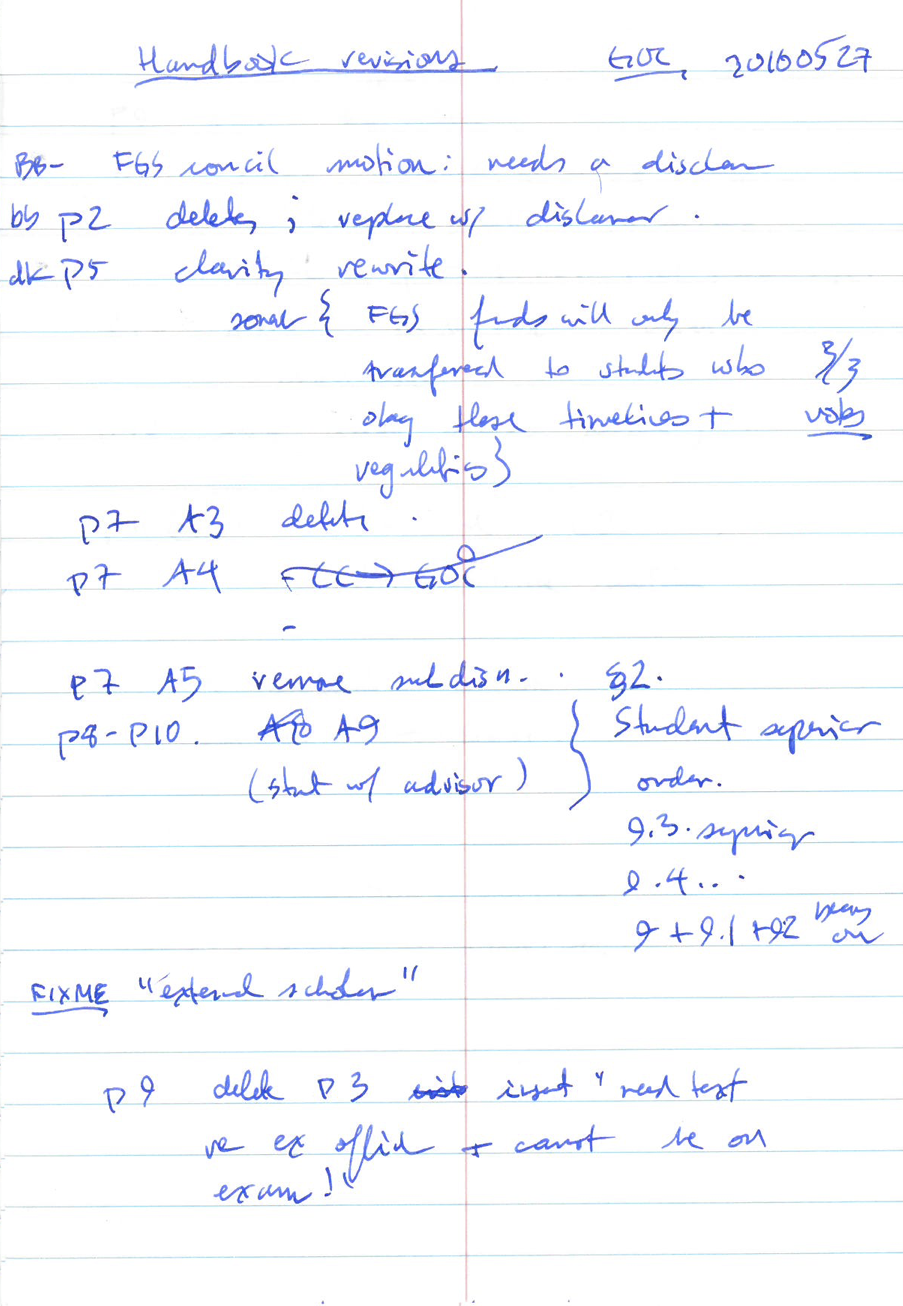
\includegraphics[height=8in]{meetings/20160527/20160527_meeting_notes_page_1.png}
% \newpage
% 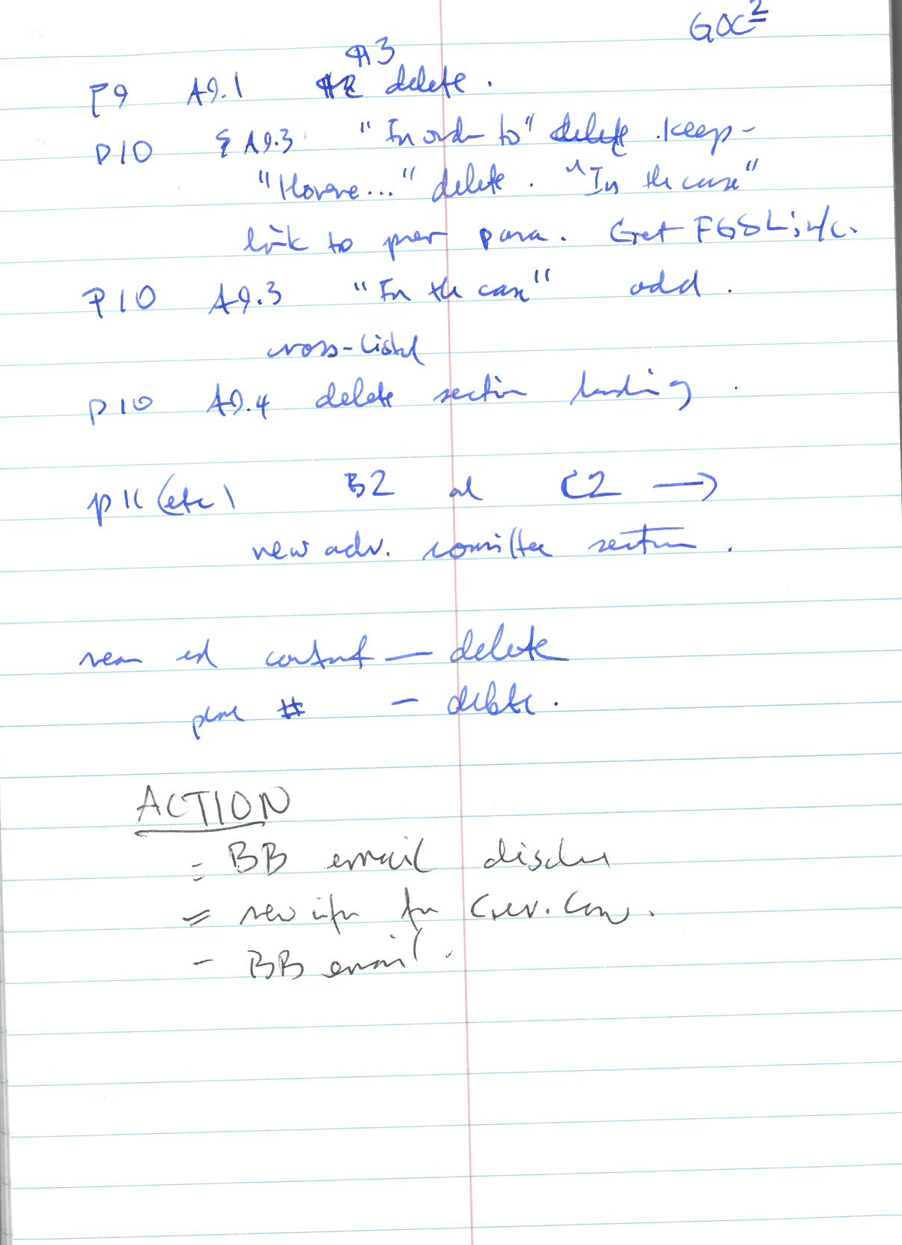
\includegraphics[height=8in]{meetings/20160527/20160527_meeting_notes_page_2.png}
% 
% \newpage
% \textbf{\large DK notes from GOC meeting on 2016-06-12} \label{mn:20160612}
% 
% 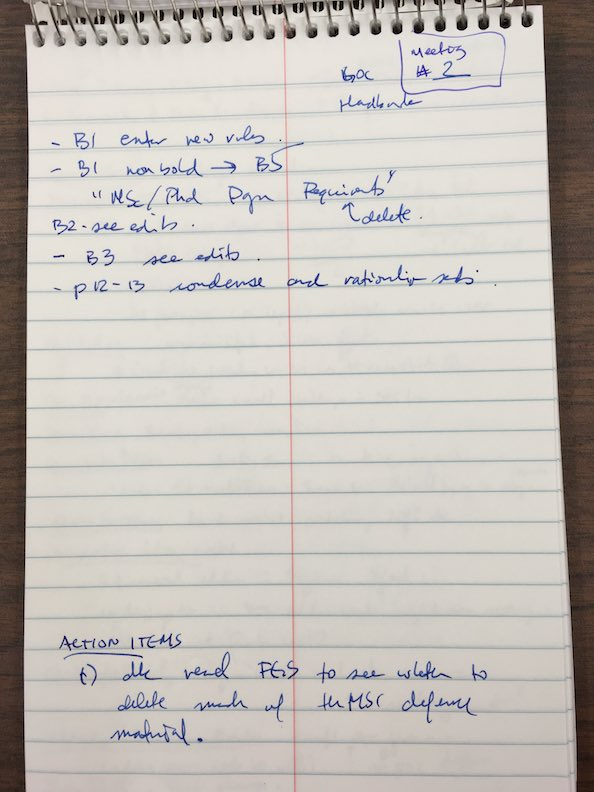
\includegraphics[height=8in]{meetings/20160612/20160612_meeting_notes.jpg}
% 
% \newpage
% \textbf{\large DK notes from GOC meeting on 2016-06-17} \label{mn:20160617}
% 
% 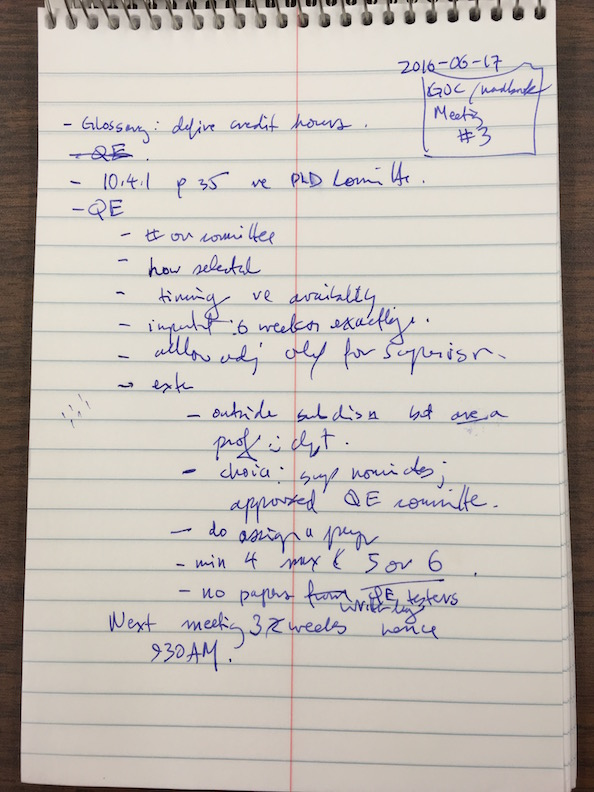
\includegraphics[height=8in]{meetings/20160617/20160617_meeting_notes.jpg}
% 
% \newpage
% \textbf{\large DK notes from GOC meeting on 2016-07-08} \label{mn:20160708}
% 
% 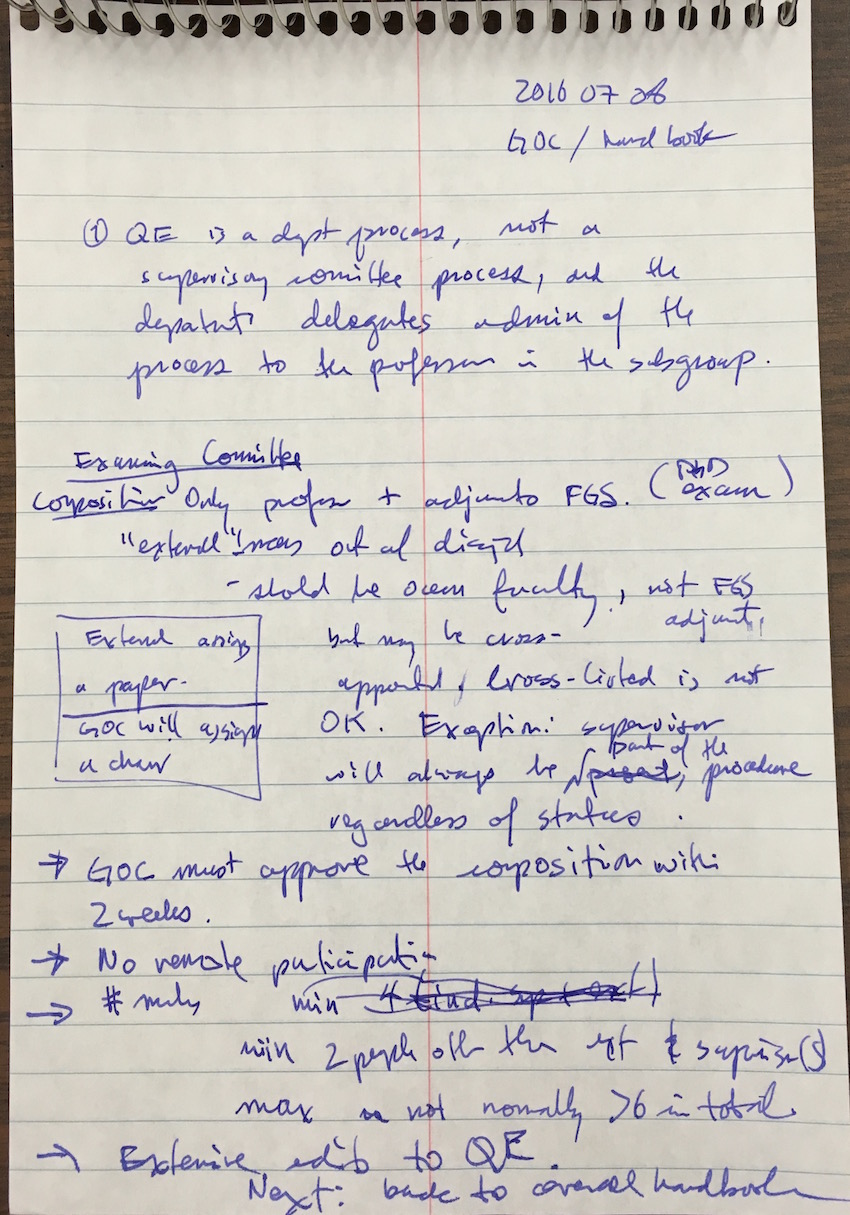
\includegraphics[height=8in]{meetings/20160708/20160708_meeting_notes.jpg}
% 
% \newpage
% \textbf{\large BioOce QE rules, marked up by DK} \label{boqe}
% 
% 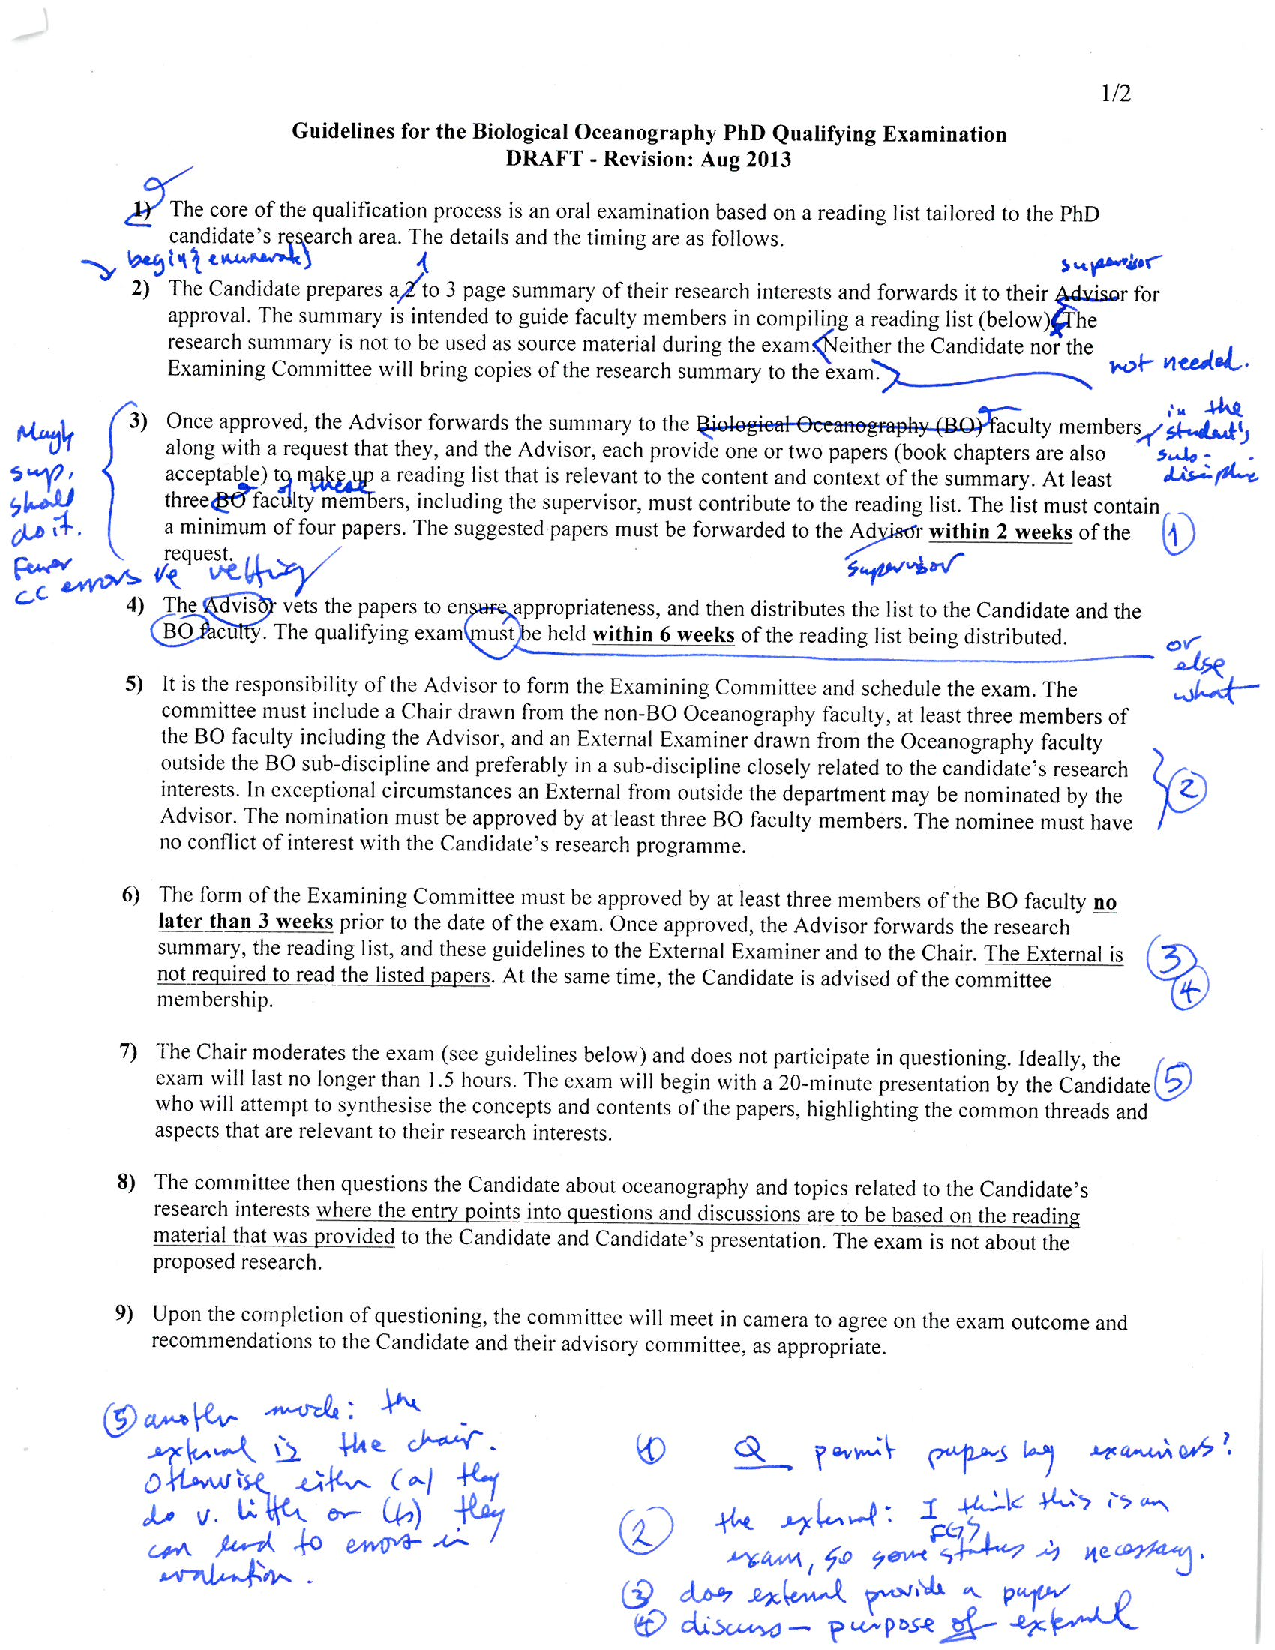
\includegraphics[height=8in]{marked_up_versions/bo_qe_20160708.pdf}


%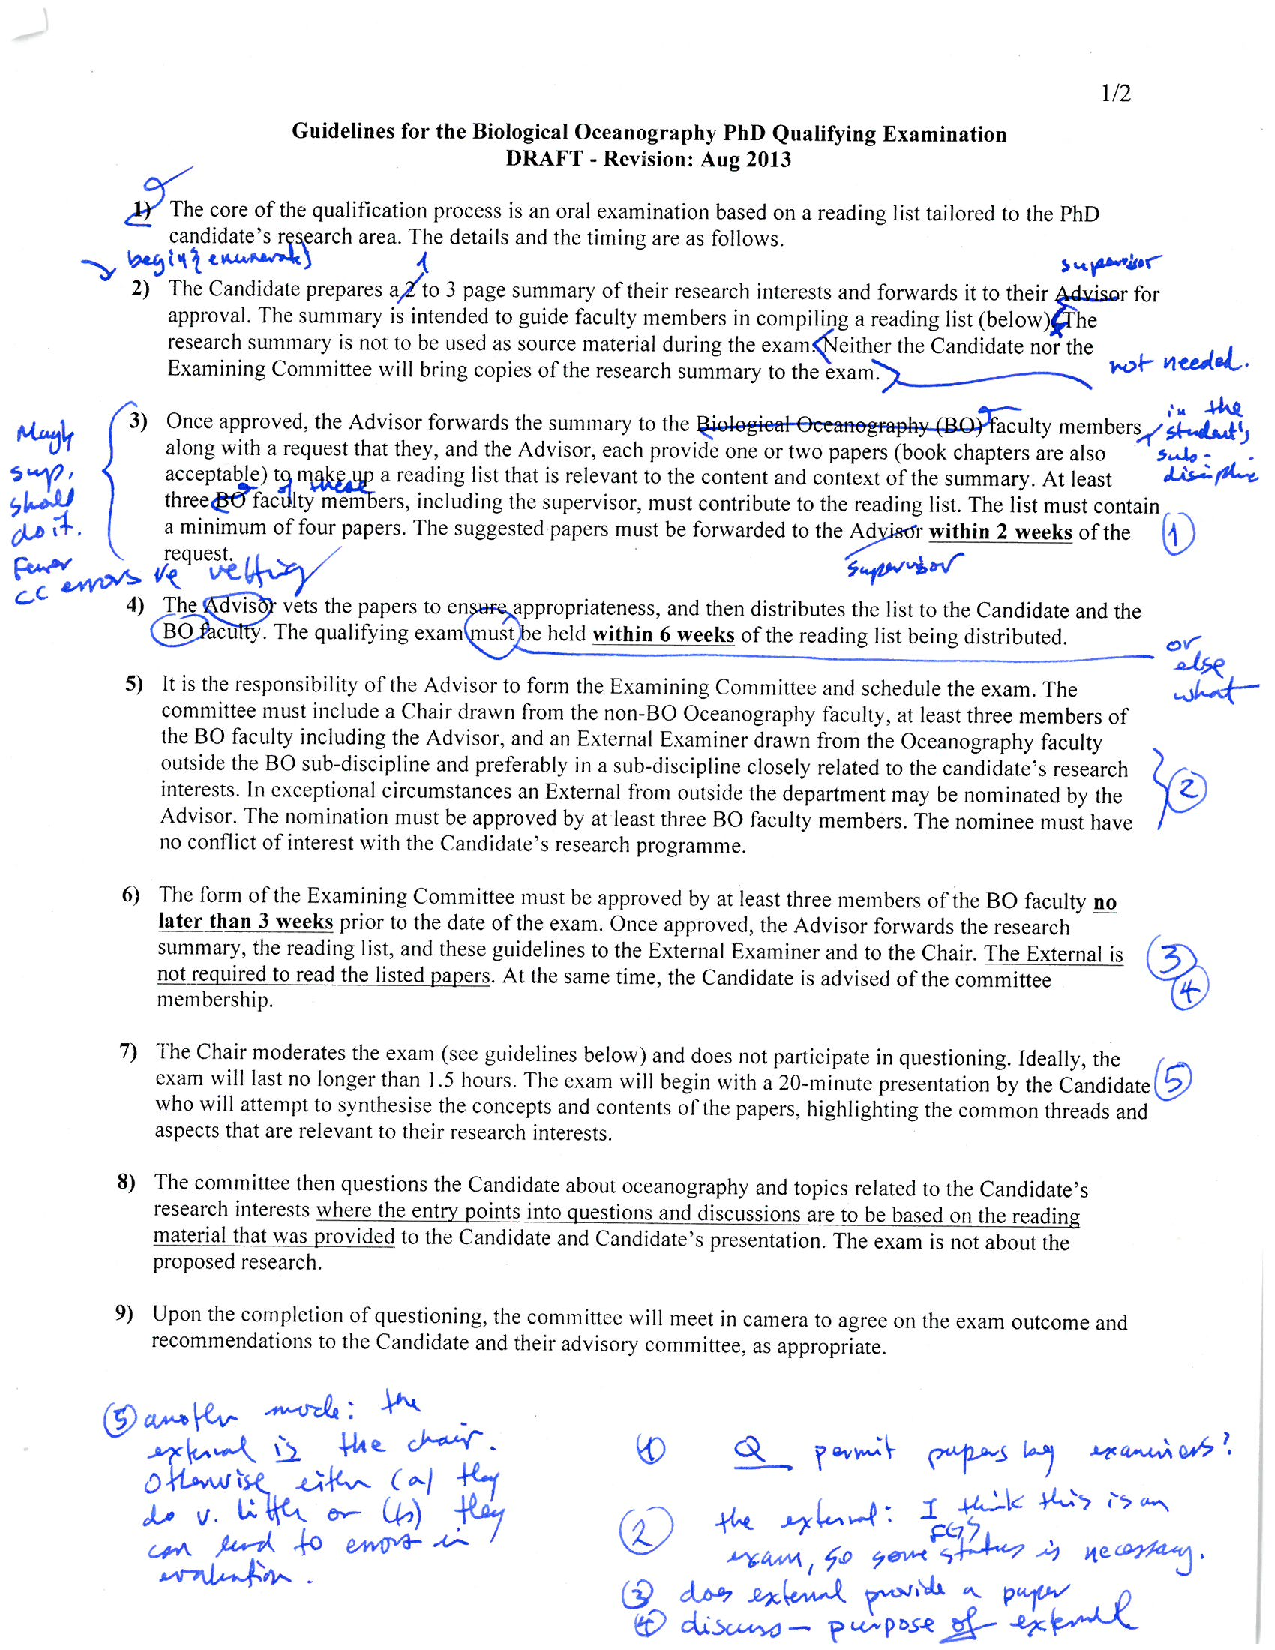
\includegraphics[height=8in]{marked_up_versions/bo_qe_20160708.pdf}


\end{document}
